% !TeX document-id = {22bc6cb6-db19-47fd-9753-6b9a7e372523}
%!TEX TS-program = pdfLaTeX
%!TEX encoding = utf-8
%!TEX spellcheck = en-US

\documentclass[12pt,twoside,openright]{article}

%nœud

%\usepackage{soul}

%\documentclass[a4paper,11pt]{book}
\usepackage[T1]{fontenc}
\usepackage[utf8]{inputenc}
%\usepackage[francais]{babel}

\usepackage{natbib}

\usepackage[usenames,dvipsnames]{color}

\usepackage{lmodern}
%%%%%%%%%%%%%%%%%%%%%%%%%%%%%%%%%%%%%%%%%%%%%%%%%%%%%%%%%
% Source: http://en.wikibooks.org/wiki/LaTeX/Hyperlinks %
%%%%%%%%%%%%%%%%%%%%%%%%%%%%%%%%%%%%%%%%%%%%%%%%%%%%%%%%%
\usepackage{hyperref}
\usepackage{graphicx}
\usepackage{pdfpages}
\usepackage{amsmath}
\usepackage{amssymb}
\usepackage{a4}
\usepackage{indentfirst}
\usepackage{fancyhdr}
\usepackage{varioref}
\usepackage{makeidx}

%\usepackage{biblatex}
%\usepackage{mslapa}

\usepackage[normalem]{ulem}

\usepackage{algorithm}
\usepackage{algorithmic}

%% Apalike hyphenation %%%
%\let\oldbibitem=\bibitem
%\renewcommand{\bibitem}[2][]{\oldbibitem[#1]{#2}\newline}

%%% Margins %%%
\voffset -2.54cm
\textheight 24cm
\hoffset -1.3in
\evensidemargin 2.5cm
\oddsidemargin 2.5cm
\textwidth 18cm

% Book's title and subtitle
%\title{\textbf{Fovea-based Scene Decoding under Variational Predictive Control}}
\title{\textbf{Fovea-based Scene Decoding through Computationally-effective Model-based Prediction}}
% Author
\author{\textsc{Emmanuel Daucé}\\
	Ecole Centrale de Marseille,\\ 
	Aix Marseille Univ, Inserm,\\ 
	INS, Institut de Neurosciences des Systèmes, \\
	Marseille, France\\
	\texttt{emmanuel.dauce@centrale-marseille.fr} 
}%\thanks{\url{www.example.com}}}
\date{}
\makeindex

\begin{document}
	
\maketitle
	
\begin{abstract}
{\color{Purple} What motivates action in the absence of a definite reward function? Considering the case of saccadic visuomotor control, we consider an apparently simple control problem that is how select the next saccade, in a sequence of discrete eye movements, when the final objective is to better interpret the current visual scene.
%An original scene decoding setup is developed here, that, accordingly with previous setups, optimizes the decoding through selecting relevant sensory samples under model-based prediction. 
The visual scene is modeled here as a partially-observed environment,
%with the current view interpreted as a mixture of two conjugate emitters, namely the ``controlled'' emitter (i.e. the actuator state), and the ``uncontrolled'' one (i.e. the latent state). 
under a generative probabilistic model explaining how the visual data is shaped by action.
This allows to interpret different action selection metrics proposed in literature, 
including the Salience, the Infomax and the Variational Free Energy, under a single information theoretic construct, namely the viewpoint-update-based Information Gain.
Pursuing this analytic track, two original metrics named the Information Gain Lower Bound (IGLB) and the Information Gain Upper Bound (IGUB) are then proposed. Showing either a conservative or an optimistic bias regarding the Information Gain, they strongly simplify its calculation.
An artificial fovea-based visual scene decoding setup is then developed, }
with numerical experiments highlighting different aspects of the setup. 
A first and principal result is that state-of-the-art recognition rates can be obtained with sequential fovea-based computing, using less than 10\% of the original signal. Those satisfactory results illustrate the advantage of mixing predictive control with accurate state-of-the-art predictors, namely a deep neural network. 
A second result is the sub-optimality of some classical metrics widely used in literature, that is not manifest with finely-tuned generative models, but becomes patent when coarse or faulty models are used.
Last, a computationally-effective predictive model is developed using the {\color{Purple}IGLB} objective, with pre-processed saccade trajectories read-out from memory, bypassing computationally-demanding predictive calculations.  This dramatically simplified setup is shown effective in our case, showing both competitive decoding compression rates and a good robustness to model flaws. 

\end{abstract}
\section{Introduction}

In complement with goal-oriented activity, animal motor control also relates to the search for sensory cues in order to better interpret its sensory environment and improve action efficacy. This resorts to choosing relevant viewpoints, i.e. selecting body placement and/or sensors orientation in order to capture a sensory signal that should help disambiguate the current scene. It corresponds to selecting views (from a large range of possible views) in order to maximize scene understanding under limited resources constraints. This task is the one considered in this paper (further on called the \emph{sensory scene decoding} task). 

Superior vertebrates oculo-motor activity typically underlies such a decoding task. The important redundancy present in the visual data was exploited by natural selection, ending up in a combination of energy-efficient sensors and resource-saving visuo-motor control, exploiting only little portions of the visual environment to decode the total sensory scene. A salient feature of superior vertebrates visual apparatus is indeed their anisotopic visual sensor, that concentrates  photoreceptors over a small central portion of the retina : the fovea \citep{osterberg1935topography}. Then, by moving the gaze with the eyes, the center of sight is constantly and actively moving around during all waking time. 
This scanning of the visual scene is principally done with high-speed targeted eye movements called saccades \citep{yarbus1967eye}, that sequentially capture local chunks of the visual scene. This makes the oculo-motor activity an essential element of man and animal behavior, underlying most of daily displacements, movements, instrumental and social interactions. 

Scene decoding through action (or ``active perception'') has attracted strong interest in robotics and artificial vision, for the important redundancy present in the sensory data allows to envisage energy-efficient  exploring devices using  little portions only of the total sensory scene.
The opportunity to neglect large parts of the sensory scene should mainly be considered when the energy is scarce, as it is the case for drones and robots. 
It is also relevant in computer vision, where mega-pixel images appeals for selective convolutions, in order to avoid unnecessary matrix products. 
The example of animal vision thus encourages a more parsimonious approach to robotic and computer vision, \emph{including the control of the sensory flow}. 
Optimizing the sensor displacements across time may then be a part of robotic control, in combination with goal-oriented operations. 

Changing the viewpoint can be seen as a way to leverage ambiguities present in the current visual field. In \citet{aloimonos1988active}, the authors show that some ill-posed object recognition problems become well-posed as soon as several views on the  same object are considered. A more general perspective is developed in \citet{bajcsy1988active}, with a first attempt to interpret active vision in the terms of sequential Bayesian estimation:
\begin{quote}
	\emph{The problem  of Active Sensing can be stated as a problem of controlling strategies 
		applied to the data acquisition process which will depend on the current state 
		of the data interpretation and  the  goal  or the  task of  the  process.}
\end{quote}
thus providing a roadmap for the development of active vision and sensory systems.

Work on central vision control is quite scarce until the late 2000's.
On the machine learning side, an example of fovea-based visuo-motor control was  addressed in \citet{schmidhuber1991learning}, with a direct policy learning from gradient descent by using BPTT through a pre-processed forward model. 
On the biological  side, early models from the late nineties  consider the case of fovea-based image encoding, ending up in the simplified ``pyramidal'' focal image encoding model \citep{kortum1996implementation}. Active vision models were however largely dominated by the \emph{salience} models \citep{itti2000saliency, itti2001computational, itti2005bayesian}, that were shown consistent with the preferred fixation zones observed in humans. 
Motor control were however generally bypassed in that case, putting the focus on characterizing the attractiveness of fixation zones rather that explaining 
the image decoding process when changing gaze orientation.
Combined with a focal pyramidal image encoding, the salience approach still provides effective outcome in image and video compression  \citep{wang2003foveation,guo2010novel}.


The salience approach to active vision is generally referred as a ``bottom-up'' approach, for only low-level aspects of the images are considered in the model. In contrast, scene interpretation and active object search in images is generally referred as the ``top-down'' approach, with high level assumptions (the ``belief'') made over the actual content of the image. 

Two parallel research tracks adopted and refined this last idea over the last twenty years.
On the one side, human visual search modeling considers the visual scan-path as a sequential \emph{sampling} of an underlying (covert) sensory scene, given a generative model. 
Stemming from \citep{bajcsy1988active}'s intuition, a \emph{predictive} approach to perception-driven control was originally developed in \citep{najemnik2005optimal} to implement this idea.
It globally complies with the predictive coding framework \citep{rao1999predictive} with the current posterior estimate used to anticipate future sensations. 
Here, appropriate samples should be selected that maximize the expected \emph{decoding accuracy}, that resorts to reduce the number of possible interpretations of the underlying scene, i.e. reduce the expected posterior \emph{entropy} (see \citet{najemnik2005optimal,najemnik2009simple,butko2010infomax,friston2012perceptions}).
More generally, the idea of having many (i.e. a mixture of) models to identify a scene complies with the weak classifiers evidence accumulation principle developed in computer vision (see \citet{viola2003fast} and sequels). It also generalizes to the case of multi-view selection in object search and scene recognition \citep{potthast2016active}.

A second research track insists on the formal contribution of action in the \emph{encoding} of the (future) sensory field. This resorts to consider action as a \emph{code} that is later on revealed (decoded) by sensing the effect of action at the visual field \citep{klyubin2005empowerment,tishby2011information}. As such it may be optimized so as to maximize the action read-out capability, allowing to improve both the policy and the data model in the course of learning \citep{schmidhuber2007simple,mohamed2015variational,houthooft2016vime}.


Those different approaches interestingly conduct to develop different objective functions that do not appear mutually compatible in a first place.
The sampling efficacy objective encourages actions that provide a consistent belief update, measured at the log likelihood of the data after sampling. This implies to avoid surprising data and prefer actions that bring out a sensory input that is consistent with the initial guess \citep{friston2010free}. This  approach may be referred as the ``conservative'' approach to action selection.  
Conversely,{ \color{Purple} the action decoding efficacy objective encourages actions that are well discriminated, i.e. that have a visible effect on the sensors. This is formally quantified by the ``empowerment'' information gain objective \citep{klyubin2005empowerment,tishby2011information}, maximizing the ``effect-of-action'' at the sensors, or by the more informal measures of surprise, like the ``Salience'' metric \citep{itti2005bayesian}, or the
different ``curiosity'' metrics, like the ones proposed in \citet{schmidhuber1991curious,oudeyer2008can, pathak2017curiosity}}. This second approach may be referred as the ``progressive'' approach to action selection. 

{\color{Purple} Perception-driven action selection is thus in need for clarification in order to develop effective action-selection controllers in open environments. This article is an attempt to develop an unifying framework, allowing both formal and quantitative comparisons between the different action selection metrics at stake under a single setup, that is choosing the next saccade in a sequential visual scene decoding task.
	
A general scene decoding setup is first developed in section \ref{sec:three-party}, under predictive control assumptions, 
with a generative probabilistic model explaining how the observed data is generated from action. 
Stemming from a partially observed framework, the current observation is interpreted as the realization of a \emph{mixed emission density} made of a controlled emitter (i.e. the actuator state) and an uncontrolled one (i.e. the latent state of the environment). Then, when combined with a chain rule-based sequential update, it is shown how the (unobserved) latent state shall be inferred from both the current observation and past inferences memory. Given that ``mixed'' generative model, a generic active inference framework is developed in section \ref{sec:perception-driven-control}, with classical action selection metrics recast, showing a clear formal separation between the ``Accuracy-based'', ``Innovation-based'' and ``Conservation-based'' action-selection metric families. 

Section \ref{sec:results} gathers  both formal and simulation results, providing a comprehensive and consistent interpretation of most existing metrics as maximizing the viewpoint update-based Information Gain, either in an ``optimistic'' or in a ``pessimistic'' fashion. The connection between action-selection metrics and the Information Gain is first formally unfolded in section \ref{sec:info-gain}.  It is shown that a rather straightforward approximation of the Information Gain,
known as the Compression Improvement, provides both a general setup to interpret most classic objective functions, and a baseline to provide effective and  principle-grounded objective functions, namely the Information Gain Lower Bound (IGLB) and the Information Gain Upper Bound (IGUB).
Then an actual implementation of a saccadic fovea-based scene decoding setup
is developed in section \ref{sec:visual-scene-dec}, allowing to quantitatively compare those different metrics, and propose new avenues toward more parsimonious scene decoding through computationally-effective model-based prediction.}


\section{Material and methods} \label{sec:material}

We consider here a \emph{scene decoding task} where an agent has to estimate its environment state, here called the ``sensory scene'', from sensory samples. The visual scene is organized in objects (or objects parts), whose presence and position is continuously checked by visual inspection. 
Then, decoding a visual scene through saccades consists in identifying the ensemble through the sequential foveation of parts of the scene only. 

\subsection{A mixed emission generative model}\label{sec:three-party}

%A ``viewpoint emitter'' $\boldsymbol{u}$ is here interpreted as both the realization of a \emph{sampling} (of an underlying generative model), and as a \emph{code} that participates in generating the incoming sensory data.
{\color{Purple} The active inference approach relies on a longstanding history of probabilistic modelling in signal processing and control \citep{Kalman1960,Baum1966}. The physical world takes the form of a random  process that is the cause of the sensory stream. This process is not visible in itself but only sensed through (non reliable) sensors, providing a sequence of observations over time. The inference problem consists in identifying the cause of the observations (i.e. the state of the environment), given the generative model. The result of the inference is itself a probability density over the hidden states (the posterior probability), that is obtained through  inverting the model (from the observations toward the hidden states).}

\subsubsection{One scene, many views}

A feedback control framework is composed of an actor and an environment. The actor and the environment interact according to a feedback loop. 
The actor can act on the environment through its effectors, and sense the state of the environment through its sensors. 
The state of the environment as well as the state of the agent can change over time. The state of the environment is described by a state vector $\boldsymbol{s} \in \mathcal{S}$.
The signal $\boldsymbol{x}$ that is measured on the sensors is called the \emph{sensory field}. It is interpreted as a measure made by the sensors, that is causally related to the current state $\boldsymbol{s}$. 

We consider here an organization of the environment in objects (or object parts), whose presence and position is continuously checked by sensori-motor inspection.
{\color{Purple} 
% a probabilistic view, $\boldsymbol{x}$ is a realization of a random variable $X$ and $\boldsymbol{s}$ is a realization of a random variable $S$.
%	The dependence between $S$ and $X$ is reflected in a joint probability distribution:
%	$\text{Pr}(X,S)$, that is said the \emph{generative model}, embedding the cause of the sensory field.
In a (discrete) Markovian framework, the state $\boldsymbol{s}$ in which the physical system is found at present depend both on its previous state (say $\boldsymbol{s}_0$) and on a preceding motor command $\boldsymbol{a}$.
The transition from $\boldsymbol{s}_0$ to $\boldsymbol{s}$ is reflected in a \emph{transition} probability that embodies the deterministic and non-deterministic effects of the command $\boldsymbol{a}$ in the form of a conditional probability:  
\begin{align}
\boldsymbol{s} \sim \text{Pr}(S|\boldsymbol{a},\boldsymbol{s}_0) \label{eq:process}
\end{align}
%implemented with a probability density function 
%$p_\text{\sc trans}(\boldsymbol{s}|\boldsymbol{a},\boldsymbol{s}_0)$.


The signal $\boldsymbol{x}$ measured on the sensors is interpreted as an effect of the current state $\boldsymbol{s}$. Once again the deterministic and non-deterministic effects are reflected in a conditional probability:
\begin{align}
\boldsymbol{x} \sim \text{Pr}(X|\boldsymbol{s})\label{eq:measure}
\end{align}
that is said the \emph{sensory emission} process.
%implemented with a probability density function 
%$p_\text{\sc meas}(\boldsymbol{x}|\boldsymbol{s})$.
The combination of  (\ref{eq:process}) and (\ref{eq:measure}) is the \emph{generative process} that is the cause of the sensory field.}
{\color{Purple} Consider now} the cause $\boldsymbol{s}$ of the current visual field $\boldsymbol{x}$ is both the object identity $\boldsymbol{o}$, its position in the peripersonal space $\boldsymbol{y}$, and the current body orientation  $\boldsymbol{u}$, i.e. $\boldsymbol{s} = (\boldsymbol{y},\boldsymbol{o},\boldsymbol{u})$, with $\boldsymbol{x} \sim \text{Pr}(X|\boldsymbol{y},\boldsymbol{o},\boldsymbol{u})$ {\color{Purple}the  sensory emission. Here} each variable accounts for a distinct degree of freedom {\color{Purple} responsible for the sensory emission}. This description of the sensory emitter as a three degrees of freedom construct is called here the ``\emph{three-party}'' emission model.

Then we propose to split the {\color{Purple} emission} process in two parts, namely the controlled {\color{Purple} emission} process and the uncontrolled {\color{Purple} emission} process. 
This separation 
is consistent with the ``hidden state''/``hidden control'' distinction stated in \citep{friston2012perceptions}.
The controlled emitter is $\boldsymbol{u}$ while the uncontrolled emitter is  $(\boldsymbol{y}, \boldsymbol{o})$. 
Moreover, for greater simplicity, $(\boldsymbol{y},\boldsymbol{o})$ is here reduced to a single variable $\boldsymbol{z} = (\boldsymbol{y}, \boldsymbol{o})$, 
so that the generic uncontrolled variable $\boldsymbol{z}$ may report for every possible composition of object identity in space (or more generally every composition of a pose and an identity).
The controlled emitter $\boldsymbol{u}$ refers to the state of a motor apparatus, e.g. to the spatial distribution of the different mobile segments of an articulated body. The uncontrolled latent emitter $\boldsymbol{z}$  refers to the remaining part of the physical world, i.e. the ``environment''. 

This restricted setup, that separates a body and an environment in the form of two {\color{Purple}independent} processes,  provides a substantial simplification to the estimation problem at stake: 
\paragraph{(i) Emitters independence}
A first assumption is that two {\color{Purple} transition processes} are independent, i.e. $\text{Pr}(Z,U) = \text{Pr}(Z)\text{Pr}(U)$ so that:
\begin{align}
(\boldsymbol{z},\boldsymbol{u}) \sim \text{Pr}(Z,U|\boldsymbol{a}, \boldsymbol{z}_0, \boldsymbol{u}_0) = \text{Pr}(Z|\boldsymbol{a}, \boldsymbol{z}_0, \boldsymbol{u}_0) \text{Pr}(U|\boldsymbol{a}, \boldsymbol{z}_0, \boldsymbol{u}_0)\nonumber
\end{align}
	
\paragraph{(ii) End-effector control}
An additional assumption is that the controlled {\color{Purple} transition} process is relatively ``fast'' in comparison with the uncontrolled one
(for, e.g, saccades can be realized in a 100-200 ms interval). 
In consequence we assimilate the motor command $\boldsymbol{a}$ with a setpoint (or posture) $\boldsymbol{u}$ in the actuator space, that is supposed to be reached 
at short notice by the motor apparatus once the command is emitted, under classical stability/controllability constraints.
This entails that, consistently with the `end-effector'' ballistic control setup \citep{mussa2004neural},  \emph{$\boldsymbol{u}$ is independent from $\boldsymbol{u}_0$},
i.e.:
\begin{align*}
\boldsymbol{u}\sim\text{Pr}(U|\boldsymbol{a})
\end{align*}

The motor command $\boldsymbol{a}$ then corresponds to the desired end-orientation of the sensor,
here considered as a setpoint in the actuators space, 
either expressed in actuators or endpoint coordinates (with hardware-implemented detailed effector response function).  
Under that perspective, the effector acts on the sensors position and orientation so as to achieve a certain perspective (or view) over the external scene, and the controlled emitter $\boldsymbol{u}$ is now called a \emph{viewpoint}. 

\paragraph{(iii) Uncontrolled environment}
The third important assumption is that the motor command $\boldsymbol{a}$ \emph{is not expected to affect the uncontrolled latent emitter $\boldsymbol{z}$}, i.e.
\begin{align*}
\boldsymbol{z} \sim \text{Pr}(Z|\boldsymbol{z}_0)
\end{align*}
so that $\boldsymbol{z}$ should depend only on the external dynamics (the external ``uncontrolled'' process).

\paragraph{(iv) Static assumption}
Under a scene decoding  task, 
it is rather common to consider the environment as ``static'' \citep{butko2010infomax}. This fourth assumption means, in short, that:
$$\text{Pr}(Z|\boldsymbol{z}_0) = \delta(Z, \boldsymbol{z}_0)$$ 
with $\delta$ the Knonecker symbol. 
The uncontrolled latent emitter $\boldsymbol{z}$ is thus expected to capture all relevant information about the current scene, while remaining invariant throughout the decoding process.


Last, the {\color{Purple}observation} $\boldsymbol{x}$ may rely on both emitters $\boldsymbol{z}$ and $\boldsymbol{u}$, i.e. 
\begin{align}
\boldsymbol{x} \sim \text{Pr}(X|\boldsymbol{z}, \boldsymbol{u})
\label{eq:gen}
\end{align} 
Each {\color{Purple}observation} $\boldsymbol{x}$ is generated from a mixed emitter $(\boldsymbol{z}, \boldsymbol{u})$, with $\boldsymbol{u}$ the controlled part of the emitter and  $\boldsymbol{z}$ the uncontrolled part. Note that $\boldsymbol{z}$ is said the latent state out of habit, though both $\boldsymbol{u}$ and $\boldsymbol{z}$ contribute to the generation of $\boldsymbol{x}$.

For notational simplicity, we absorb here the execution noise \citep{van2004role} in the measure process, i.e.:
$\boldsymbol{x} \sim \text{Pr}(X|\boldsymbol{z}, U)\text{Pr}(U|\boldsymbol{a})$.
Then, by notational abuse, we assimilate in the rest of the paper  $\boldsymbol{u}$ (the controlled emitter) with $\boldsymbol{a}$ (the motor command), so that 
a single variable $\boldsymbol{u} \equiv \boldsymbol{a}$ should be used for both. %We also call the uncontrolled latent emitter $\boldsymbol{z}$ the \emph{latent state} for simplicity.
Each different $\boldsymbol{u}$ is thus both interpreted as a
motor command and as {\color{Purple} an emitter}. As a motor command, it is controllable, i.e. determined by a controller. As {\color{Purple} an emitter}, it monitors the generation of the sensory field, in combination with the latent state $\boldsymbol{z}$. 

Finally, both $\boldsymbol{x}$ (the view) and $\boldsymbol{z}$ (the \emph{latent state}) are the realization of a generative model parametrized by $\boldsymbol{u}$, i.e.
\begin{align}
\boldsymbol{x}, \boldsymbol{z} | \boldsymbol{u} \sim \text{Pr}(X|Z, \boldsymbol{u}), \text{Pr}(Z) \label{eq:generative}
\end{align}  
with $\text{Pr}(Z)$ the \emph{prior}, and each different motor command $\boldsymbol{u}$ providing a different sample over the same underlying distribution. Under that prospect, the action $\boldsymbol{u}$ is interpreted as a \emph{sampling} operation.

\subsubsection{Sequential Bayesian inference}\label{sec:seq-bayes}


With a generative model comes the possibility to \emph{infer} the latent state of the physical system {\color{Purple} from the observation}
using Bayes rule:
\begin{align}
\text{Pr}(Z|\boldsymbol{x},\boldsymbol{u})
= \frac{\text{Pr}(\boldsymbol{x}|Z, \boldsymbol{u}) \text{Pr}(Z)}
{\text{Pr}(\boldsymbol{x}|\boldsymbol{u})}\label{eq:post-Pr}
\end{align}
with $\text{Pr}(Z|\boldsymbol{x},\boldsymbol{u})$ the \emph{posterior} probability
(over the latent states), whose order 2 moment informs on the estimation accuracy : the narrower the distribution, the more accurate the latent state prediction. 

{\color{Purple} In a visual scene decoding task, a single environment state $\boldsymbol{z}$ is
observed through a series of viewpoints $\boldsymbol{u}$, $\boldsymbol{u}'$, $\boldsymbol{u}''$, ... This sequence of observations should ultimately provide a final estimate $\hat{q}(Z)$, with a single cause $\hat{\boldsymbol{z}}$ dominating the other ones, allowing to reach a final decision. }
%This is the \emph{scene decoding} task we analyze next.
The chaining of the posterior to the role of the prior in the next inference step is a classical property of sequential Bayesian inference.
When generalized to many observations: $(\boldsymbol{x}|\boldsymbol{u}), (\boldsymbol{x}'|\boldsymbol{u}')$, ..., $(\boldsymbol{x}^{(n)}|\boldsymbol{u}^{(n)})$, the final posterior $q^{(n)}(Z)$ writes:
\begin{align}
q^{(n)}(Z) \propto \text{Pr}(\boldsymbol{x}|Z,\boldsymbol{u}) \times \text{Pr}(\boldsymbol{x}'|Z,\boldsymbol{u}') \times ... \times \text{Pr}(\boldsymbol{x}^{(n)}|Z,\boldsymbol{u}^{(n)}) \times \text{Pr}(Z) \label{eq:accum}
\end{align}
which allows to approach the latent state $\boldsymbol{z}$ from many samples of (\ref{eq:gen}), each sample providing more evidence. 
{\color{Purple} When the sampling is done incrementally \citep{wald1945sequential},}
the $\boldsymbol{u}$'s and $\boldsymbol{x}$'s do not need to be stored in the process. At step $n$, only $q^{(n-1)}$ (the current ``belief'') needs to be memorized to estimate $q^{(n)}$, i.e. 
\begin{align} 
q^{(n)}(Z) \propto \text{Pr}(\boldsymbol{x}^{(n)}|Z,\boldsymbol{u}^{(n)}) \times q^{(n-1)}(Z) \label{eq:accum-post}
\end{align}

\subsection{Predictive control and action selection metrics}\label{sec:perception-driven-control}

%\subsubsection

Consider an agent having to estimate its environment state $\boldsymbol{z}$ from sampling it from different viewpoints. We here suppose that a generative model $p$ is given to the agent. 
Depending on  the current viewpoint $\boldsymbol{u}$, a different view $\boldsymbol{x}$ is observed at the sensors. So, each different command $\boldsymbol{u}$ provokes a different observation, and thus a different 
estimation of the latent state. It is thus worth to question what is the optimal choice for $\boldsymbol{u}$ in order to maximize the accuracy of the posterior estimate?
That turns  to minimize the number of samples so as to provide an accurate estimate. This approach to inference is called \emph{active sampling} in \citet{friston2012perceptions}, for the choice of $\boldsymbol{u}$ determines the sensory sample $\boldsymbol{x}$ that is observed, conditioning the final posterior estimate. {\color{Purple} It was originally developed by \citet{najemnik2005optimal} to the case of human visual search modelling (finding a target feature in an image, i.e. the ``find Waldo'' task).}

A baseline sampling strategy is to choose $\boldsymbol{u}$ at random and condition the posterior  estimate on this random action. 
More elaborate strategies consider the past observations
to choose the most promising action $\hat{\boldsymbol{u}}$. %We have seen in  
The knowledge about past observations being here absorbed in single posterior distribution $q^{(n-1)}$, the problem turns out to design  a \emph{controller} $C$ which, given a context $q^{(n-1)}$, sets up an action $\hat{\boldsymbol{u}} = C(q^{(n-1)})$. Here the role of the controller is not to achieve a goal-oriented task, but to render the estimation of the latent state more accurate. The controller is said \emph{perception-driven}. 

The design of such a controller is not straightforward. On contrary to classical control, there is not definite setpoint $\boldsymbol{z}^*$ to which the controller is supposed to drive the external process (through model inversion for instance). By design, the actual latent state $\boldsymbol{z}$ is not visible as such and can not be compared to the inferred posterior. In order to estimate how good a motor command is, one needs to provide an estimate of the value-of-action (regarding scene understanding). There is currently no consensus about what a good value is regarding the scene decoding task. 

A general strategy is thus to establish an {\color{Purple} \emph{action selection metric}, taking either the form of an \emph{objective function} $f$ or a loss $\ell$}, that conveys a quantitative estimation of the action's contribution to the inference accuracy (resp. imprecision). Once the objective function established, a simple control strategy is to choose the action that maximizes the objective (resp. minimizes the loss), i.e.:
\begin{align}
\hat{\boldsymbol{u}} = \underset{\boldsymbol{u}\in\mathcal{U}}{\text{ argmin }}  \ell(\boldsymbol{u})\left/ \underset{\boldsymbol{u}\in\mathcal{U}}{\text{ argmax }}  f(\boldsymbol{u})\right.
\end{align}
Many such objective functions are proposed in the literature. They are generally referred as an \emph{intrinsic} motivation \citep{oudeyer2008can} by contrast with the \emph{extrinsic} motivation that relates to the classical rewards in reinforcement learning \citep{sutton1998reinforcement}. {\color{Purple} Several such intrinsic reward candidates have been developed in recent years in the scene decoding context. Some of them are presented in the next paragraphs. The original formulas have been recast to show their formal correspondences, but also highlight some manifest differences between them.}

\subsubsection{Accuracy-based metrics}\label{sec:infomax}

Given a generative model $p(X,U,Z)$, like the one described in section \ref{sec:three-party}, the predictive approach to perception-driven control \citep{najemnik2005optimal} relies on predicting an \emph{accuracy} measure $A(\boldsymbol{x}, \boldsymbol{u}; q^{(n-1)})$ to choose action. 
The accuracy tells how good the model is at predicting $\boldsymbol{z}$ (here the target position) when viewing $\boldsymbol{x}$ at position $\boldsymbol{u}$,
knowing $q^{(n-1)}$ (the estimated posterior at step $n-1$).

If the agent has to choose an action $\boldsymbol{u} \in \mathcal{U}$, knowing only $q^{(n-1)}$, the \emph{predicted} accuracy attached to $\boldsymbol{u}$ is:
\begin{align*}
\bar{A}(\boldsymbol{u}; q^{(n-1)})
&= \mathbb{E}_{\boldsymbol{z} \sim q^{(n-1)}(Z), \boldsymbol{x} \sim p(X|\boldsymbol{z}, \boldsymbol{u})}\left[A(\boldsymbol{x}, \boldsymbol{u}; q^{(n-1)})\right]  \\
&= \sum_{z\in\mathcal{Z}} q^{(n-1)}(\boldsymbol{z}) \int_{\mathcal{X}}  A(\boldsymbol{x}, \boldsymbol{u}; q^{(n-1)}) p(\boldsymbol{x}|\boldsymbol{z}, \boldsymbol{u}) d\boldsymbol{x}  
\end{align*}
and the optimal action to choose is:
\begin{align}
\hat{\boldsymbol{u}} = \underset{\boldsymbol{u} \in \mathcal{U}}{\text{ argmax }} \bar{A}(\boldsymbol{u}; q^{(n-1)})\label{eq:predictive-policy}
\end{align} 
In order to render the computation tractable, a \emph{sampling} approach is generally used to estimate the predicted accuracy, i.e. $\mathbb{E}_p[f(\boldsymbol{x})] \simeq f(\tilde{\boldsymbol{x}})$, with $\tilde{\boldsymbol{x}}\sim p(\boldsymbol{x})$.

The accuracy metric used in the original paper was an ad-hoc one \citep{najemnik2005optimal}, but turned out to be consistent with minimizing the \emph{posterior entropy} \citep{najemnik2009simple}, i.e.:
$$A(\boldsymbol{x}, \boldsymbol{u}; q^{(n-1)}) = -H(q^{(n)}) = \sum_{z \in \mathcal{Z}} q^{(n)}(\boldsymbol{z}) \log q^{(n)}(\boldsymbol{z})$$
with: $q^{(n)}(\boldsymbol{z}) \propto p(\boldsymbol{x|\boldsymbol{z}, \boldsymbol{u}}) \times q^{(n-1)}(\boldsymbol{z}) $,
so that:
$$\hat{\boldsymbol{u}} = \underset{\boldsymbol{u} \in \mathcal{U}}{\text{ argmin }} \mathbb{E}_{\boldsymbol{z} \sim q^{(n-1)}(Z), \boldsymbol{x} \sim p(X|\boldsymbol{z}, \boldsymbol{u})}\left[H(q^{(n)})\right] $$ 
which makes sense for a low entropy of the posterior is expected when the estimated posterior accuracy is high.


This approach to optimal visual sampling was further on linked to an ``Infomax'' principle {\color{Purple} (posterior mutual Information Maximization)} in \citet{butko2010infomax}, 
taking:
\begin{align}A_\text{\sc infomax}(\boldsymbol{x}, \boldsymbol{u}; q^{(n-1)}) \equiv I(Z; \boldsymbol{x}|\boldsymbol{u}; q^{(n-1)})
= H(q^{(n-1)}) - H(q^{(n)})
\label{eq:infomax}
\end{align}
with  $H(q^{(n-1)}) \equiv H(Z|q^{(n-1)})$ and $H(q^{(n)}) \equiv H(Z|\boldsymbol{x}, \boldsymbol{u}; q^{(n-1)})$, {\color{Purple} which also turns out to minimize $H(q^{(n)})$ solely for $H(q^{(n-1)})$ is independent of $\boldsymbol{u}$}.
The Infomax (or posterior entropy minimization) approach generally makes sense for it implicitly relies on the chaining from $q^{(n-1)}$ to $q^{(n)}$, that considers that if $p(\boldsymbol{x}|Z, \boldsymbol{u})$ is consistent with $q^{(n-1)}(Z)$, then the issued posterior entropy should be lower than if $p(\boldsymbol{x}|Z, \boldsymbol{u})$ is at odd with $q^{(n-1)}(Z)$. The model is expected to choose the action that may confirm the initial assumption, though there is no formal comparison between $q^{(n-1)}$ and $q^{(n)}$.
It is thus potentially vulnerable to model outliers with $q^{(n)}$ having both a low entropy and being inconsistent with $q^{(n-1)}$.

\subsubsection{Innovation-based metrics}\label{sec:saliency}

Another quantity of interest is the so-called \emph{Bayesian surprise} or \emph{Salience} \citep{itti2005bayesian} defined as the Kullback-Leibler divergence  between an actual view $\boldsymbol{x}$ and a model $\boldsymbol{z}$. In the original ``bottom-up'' setup, only local statistics are formed over small image patches of a given image, with $\boldsymbol{u}$ the index of a patch and $p(\boldsymbol{z}|\boldsymbol{x},\boldsymbol{u})$ the features inferred from the data actually observed at $\boldsymbol{u}$. For each patch $\boldsymbol{u}$, the Salience of the actual view $\boldsymbol{x}$ given the model is:
$$ S(\boldsymbol{x},\boldsymbol{u}) = \text{KL}(p(Z| \boldsymbol{x}, \boldsymbol{u})||p(Z))$$
{\color{Purple} with $\text{KL}(p_1||p_2) = \sum_z p_1(\boldsymbol{z}) \log \frac{p_1(\boldsymbol{z})}{p_2(\boldsymbol{z})}$ the Kullback-Leibler divergence between $p_1$ and $p_2$, interpreted here as} a measure of the \emph{in}consistency between a (viewpoint independent)  model $p$ and the data. A high salience reflects a strong inconsistency with the model, while a low salience reflects a strong consistency with the model. According to Itti and Baldi, the regions that have a high Bayesian surprise are the ones that attract the sight the most. The calculation of $S(\boldsymbol{x}, \boldsymbol{u})$ at each location $\boldsymbol{u}$ forms a \emph{saliency map} that is then considered as a prediction of where the sight will most likely be attracted (high values most probably attract the sight, low values less probably do). The saliency model has a strong explanatory power and provides among the best fit with the actual preferred fixation zones observed in humans.
Its scalability moreover provides straightforward applications in image and video compression  \citep{wang2003foveation,guo2010novel}.

Generalized to the sequential setup, the saliency metric becomes:
\begin{align} S(\boldsymbol{x},\boldsymbol{u}; q^{(n-1)}) = \text{KL}(q^{(n)}||q^{(n-1)})\label{eq:saliency}
\end{align}
with $q^{(n-1)}$ considered as the data model and $q^{(n)}$ the posterior estimated at $(\boldsymbol{x},\boldsymbol{u})$, {\color{Purple} knowing $q^{(n-1)}$}. A corresponding predictive policy would be:
$$ \hat{\boldsymbol{u}} = \underset{\boldsymbol{u} \in \mathcal{U}}{\text{ argmax }} \mathbb{E}_{\boldsymbol{z} \sim q^{(n-1)}, \boldsymbol{x} \sim p(X|\boldsymbol{z}, \boldsymbol{u})}\left[\text{KL}(q^{(n)}||q^{(n-1)})\right]$$

\subsubsection{Conservation-based metrics}\label{sec:conservation}

At last, the  Variational Free Energy based (VFE) active inference setup \citep{friston2010free,friston2012perceptions} 
considers the general tendency of the brain to counteract surprising and unpredictable sensory events through minimizing the VFE with action (see appendix \ref{app:VFE}). In an active sampling-based setup, it writes:
\begin{align}
F(\boldsymbol{x}|\boldsymbol{u}) 
%&= \mathbb{E}_{\boldsymbol{z} \sim q} \left[-\log p(\boldsymbol{x}^{(n)}| \boldsymbol{z}, \boldsymbol{u}^{(n)} )\right] + \text{KL}(q(Z)||q^{(n-1)}(Z))
%\label{eq:FEP-prior-uxun}\\
&= -\log p(\boldsymbol{x}|\boldsymbol{u}) + \text{KL}(q(Z)||p(Z|\boldsymbol{x},\boldsymbol{u}))
\label{eq:FEP-posterior-u}
\end{align}
From the predictive perspective, stemming from $q^{(n-1)}$ as the current scene interpretation, \citet{friston2017active} propose a \emph{predictive VFE} that writes in our sequential setup like~:
\begin{align}
\bar{F}(\boldsymbol{u}; q^{(n-1)}) = \mathbb{E}_{\boldsymbol{z} \sim q^{(n-1)}(Z), \boldsymbol{x} \sim p(X|\boldsymbol{z}, \boldsymbol{u})}
\left[-\log p(\boldsymbol{x}| \boldsymbol{u}; q^{(n-1)}) + \text{KL}(q^{(n-1)}||q^{(n)})\right]
\label{eq:ELBO}
\end{align}
with $q^{(n)}$ the predicted posterior and $\text{KL}(q^{(n-1)}||q^{(n)})$ quantifying the {\color{Purple} scene interpretation update} made by interpreting  the scene with $q^{(n)}$ instead of $q^{(n-1)}$. {\color{Purple} It is said the ``epistemic cost''\footnote{or negative epistemic value.}}.
In that setup, minimizing the Free-Energy is consistent with minimizing $\text{KL}(q^{(n-1)}||q^{(n)})$
estimated as:
\begin{align*}
\text{KL}(q^{(n-1)}||q^{(n)})
&= \mathbb{E}_{\boldsymbol{z} \sim q^{(n-1)}(Z)} \left[\log q^{(n-1)}(\boldsymbol{z}) - \log q^{(n)}(\boldsymbol{z})\right]
\end{align*}

Put in a predictive form, the selection of action finally relies on reducing the predicted log ratio, i.e.~:
\begin{align}
\hat{\boldsymbol{u}} &= \underset{\boldsymbol{u} \in \mathcal{U}}{\text{ argmin }} \mathbb{E}_{\boldsymbol{z} \sim q^{(n-1)}(Z), \boldsymbol{x} \sim p(X|\boldsymbol{z}, \boldsymbol{u})}\left[\log q^{(n-1)}(\boldsymbol{z}) - \log q^{(n)}(\boldsymbol{z})\right]
\end{align}
which may {\color{Purple} minimize the \emph{epistemic cost}}\footnote{It is to be noticed  that the  Kullback-Leibler divergence is here absorbed in the general expectation over the $\boldsymbol{x}$'s and the $\boldsymbol{z}$'s.}.


On contrary to the Infomax objective (section \ref{sec:infomax}), {\color{Purple}minimizing the  epistemic cost} selects the predicted posterior having the highest consistency with the current posterior, which may prevent from model outliers that may incidently ``hack'' the posterior entropy (see section~\ref{sec:infomax}).
Minimizing $\text{KL}(q^{(n-1)}||q^{(n)})$ thus corresponds to a \emph{conservative} approach to the scene interpretation
that is \emph{minimally} vulnerable to outliers, i.e. that minimizes the risk of a {\color{Purple} conflicting} interpretation. 

The {\color{Purple} epistemic cost} is moreover at odd with the Saliency objective (section \ref{sec:saliency}) seeking the maximal \emph{in}consistency between the cumulated posterior and the current posterior.
It is obvious here that the Free Energy minimization and the Saliency maximization are antithetic objectives, and no consensus is currently observed in the literature about which objective should prevail (though Infomax generally preferred in scene decoding and saliency/surprise preferred in sparse reinforcement learning).


\section{Results} \label{sec:results}



\subsection{Information Gain based metrics}\label{sec:info-gain}
The structure of the problem (many views on the same scene) implies that {\color{Purple} different observations} should share a common information corresponding to the actual (covered) sensory scene.
We take here benefit of the {\color{Purple} view-based} variational encoding setup
{\color{Purple} (seen in section \ref{sec:conservation} and appendix \ref{app:VFE}) to propose a new quantification the \emph{mutual information} shared across different sensory fields, locally estimated with a view-based Information Gain metric. It is shown here that a rather straightforward approximation of the information gain,
	known as the Compression Improvement, provide both a general setup to interpret most classic objective functions, and a baseline to provide effective and  principle-grounded objective functions.}

%{\color{magenta} \bf When only the variations of $p$ and $q$ are considered in the optimization, each viewpoint $\boldsymbol{u}$ provides a distinct optimization problem that is resolved by finding $q(Z)\simeq p(Z|\boldsymbol{x}, \boldsymbol{u})$. 

%... ...
%}

\subsubsection{Definitions}

\paragraph{Mutual Information and Information Gain}
The sharing of information between two sensory fields $\boldsymbol{x}|\boldsymbol{u}$ and $\boldsymbol{x}'|\boldsymbol{u}'$  should be quantified by their \emph{Mutual Information}. The general idea is that two samples may provide more insight about the hidden sensory scene than a single one (three samples should provide even more, etc.). 
%Reading two co-dependent samples should also provide more guarantee about the scene interpretation than reading two independent variables.  
{\color{Purple} Consider $\boldsymbol{x}|\boldsymbol{u}$ as the initial sensory sample and $\boldsymbol{x}'|\boldsymbol{u}'$ as an additional sample providing new evidence about how interpret the initial view $\boldsymbol{x}$}.
The mutual information writes:
\begin{align}
	I((X| \boldsymbol{u}); (X'| \boldsymbol{u}')) &= H(X| \boldsymbol{u}) - H(X| \boldsymbol{u}, X', \boldsymbol{u}')\label{eq:mutual-info}\\
	&\simeq \mathbb{E}_{X,X'} \left[-\log p(X| \boldsymbol{u}) + \log p(X| \boldsymbol{u}, X', \boldsymbol{u}')\right] 
\end{align}
with :
\begin{itemize}
	\item[($i$)] $ p(\boldsymbol{x}| \boldsymbol{u}', \boldsymbol{x}', \boldsymbol{u}) \triangleq \sum_{\boldsymbol{z}} p(\boldsymbol{x}|\boldsymbol{z}, \boldsymbol{u}) p(\boldsymbol{z}|\boldsymbol{x}', \boldsymbol{u}')$ 
	the \emph{post-sample} likelihood, i.e. the retrospective likelihood of having seen $\boldsymbol{x}$ at $\boldsymbol{u}$ knowing now that $\boldsymbol{x}'$ is observed at $\boldsymbol{u}'$, and
	\item[($ii$)] 
	$-\log p(\boldsymbol{x}| \boldsymbol{u}) + \log p(\boldsymbol{x}| \boldsymbol{u}', \boldsymbol{x}', \boldsymbol{u})$ the post-sample
	\emph{Information Gain} (see also \citet{tishby2011information}), that is a local estimator of the mutual information at $X = \boldsymbol{x}$ and $X' = \boldsymbol{x}'$, {\color{Purple} given the model $p$}:
	\begin{align}
		\text{IG}(\boldsymbol{x},\boldsymbol{u}, \boldsymbol{x}', \boldsymbol{u}') 
		&= -\log p(\boldsymbol{x}| \boldsymbol{u}) + \log p(\boldsymbol{x}| \boldsymbol{u}', \boldsymbol{x}', \boldsymbol{u}) \label{eq:info-gain}
	\end{align}
\end{itemize}



\paragraph{Reconstruction Cost Update}
{\color{Purple} Stemming from the sequential Bayes posterior update formula:
	\begin{align} p(\boldsymbol{z}|\boldsymbol{x}, \boldsymbol{u}, \boldsymbol{x}', \boldsymbol{u}') = \frac{p(\boldsymbol{x}|\boldsymbol{z}, \boldsymbol{u})p(\boldsymbol{z}|\boldsymbol{x}', \boldsymbol{u}')}{p(\boldsymbol{x}|\boldsymbol{u},\boldsymbol{x}',\boldsymbol{u}')}
		%= \frac{p(\boldsymbol{x}'|\boldsymbol{z}, \boldsymbol{u}')p(\boldsymbol{z}|\boldsymbol{x}, \boldsymbol{u})}{p(\boldsymbol{x}'|\boldsymbol{u}',\boldsymbol{x},\boldsymbol{u})}
	\end{align} 
}
{\color{Purple} It can be shown that the negative log likelihood of $\boldsymbol{x}$ after seeing both $\boldsymbol{x}$ and $\boldsymbol{x}'$ is  bounded from above by}:
\begin{align}
	-\log p(\boldsymbol{x}| \boldsymbol{u}, \boldsymbol{x}', \boldsymbol{u}') 
	&\leq - \sum_z q'(z) \log p(\boldsymbol{x}| \boldsymbol{z}, \boldsymbol{u}) \frac{p(\boldsymbol{z} |\boldsymbol{x}', \boldsymbol{u}')} {q'(z)}  \nonumber\\
	&= \mathbb{E}_{\boldsymbol{z} \sim q'} \left[-\log p(\boldsymbol{x}| \boldsymbol{z}, \boldsymbol{u})\right] + \text{KL}(q'(Z)||p(Z|\boldsymbol{x}',\boldsymbol{u}'))
	\label{eq:FEP-uxu}\\
	&=  -\log p(\boldsymbol{x}| \boldsymbol{u}, \boldsymbol{x}',\boldsymbol{u}') + \text{KL}(q'(Z)||p(Z|\boldsymbol{x},\boldsymbol{u},\boldsymbol{x}',\boldsymbol{u}'))
	\label{eq:FEP-uxu2}\\
	&\triangleq F(\boldsymbol{x}|\boldsymbol{u}, \boldsymbol{x}', \boldsymbol{u}')\nonumber
\end{align}
which establishes $F(\boldsymbol{x}|\boldsymbol{u}, \boldsymbol{x}', \boldsymbol{u}')$ as the post-sample \emph{reconstruction cost} {\color{Purple} (or \emph{post-sample Free Energy} -- the two are synonyms)}, with $q'(\boldsymbol{z})$ expectedly approaching  $p(\boldsymbol{z}|\boldsymbol{x}, \boldsymbol{u}, \boldsymbol{x}', \boldsymbol{u}')$ after optimization.
From a variational perspective, the passing from $q(Z) \simeq p(Z|\boldsymbol{x}, \boldsymbol{u})$ to $q'(Z) \simeq p(Z|\boldsymbol{x}, \boldsymbol{u}, \boldsymbol{x}', \boldsymbol{u}')$ is the \emph{variational posterior update}, and the passing from $F(\boldsymbol{x}|\boldsymbol{u})$ toward   $F(\boldsymbol{x}|\boldsymbol{u}', \boldsymbol{x}', \boldsymbol{u})$ is the \emph{reconstruction cost update}. 

\paragraph{Compression Improvement}
An approximation of the Information Gain (IG), known as the \emph{Compression Improvement} (CI) was proposed in \citet{schmidhuber2007simple,houthooft2016vime}. In our setup, it
writes~:
\begin{align}
	\text{CI}(\boldsymbol{x},\boldsymbol{u}, \boldsymbol{x}', \boldsymbol{u}') = F(\boldsymbol{x}|\boldsymbol{u}) - F(\boldsymbol{x}|\boldsymbol{u}, \boldsymbol{x}', \boldsymbol{u}') \label{eq:CI-base}
\end{align}	
There comes the possibility to  {\color{Purple}optimize the \emph{next} sampling $\boldsymbol{u}'$ through maximizing the CI as a proxy for the IG. It happens 
	%from (\ref{eq:CI-base}) 
	to be equivalent with minimizing the post-sample Free Energy, consistently with \citet{friston2012perceptions}'s intuition.}

\subsubsection{Approximate Information Gain in the sequential setup}

{\color{Purple} Extending now to the sequential setup}, the contribution of $\boldsymbol{u}^{(n)}$ in understanding the scene is measured by a change in the reconstruction cost $F$ \emph{before} and \emph{after} reading $\boldsymbol{x}^{(n)}|\boldsymbol{u}^{(n)}$.
\begin{itemize}
	\item Before {\color{Purple} reading $\boldsymbol{x}^{(n)}$}, the reconstruction cost at $\boldsymbol{x}^{(n-1)}$ writes:
	\begin{align}
		F(\boldsymbol{x}^{(n-1)}|\boldsymbol{u}^{(n-1)}; q^{(n-2)}) 
		&= \mathbb{E}_{\boldsymbol{z} \sim q} \left[-\log p(\boldsymbol{x}^{(n-1)}| \boldsymbol{z}, \boldsymbol{u}^{(n-1)} )
		\right] + \text{KL}(q||q^{(n-2)}) \label{eq:F_pre_var}\\
		&= -\log p(\boldsymbol{x}^{(n-1)}|\boldsymbol{u}^{(n-1)}; q^{(n-2)}) + \text{KL} (q||q^{(n-1)})\label{eq:F_pre_KL}
	\end{align}
	\item After {\color{Purple} reading $\boldsymbol{x}^{(n)}$}, it writes:
	\begin{align}
		F(\boldsymbol{x}^{(n-1)}|\boldsymbol{u}^{(n-1)},\boldsymbol{x}^{(n)},\boldsymbol{u}^{(n)}; q^{(n-2)}) 
		&= \mathbb{E}_{\boldsymbol{z} \sim q'} \left[-\log p(\boldsymbol{x}^{(n-1)}| \boldsymbol{z}, \boldsymbol{u}^{(n-1)} )
		\right] + \text{KL}(q'||q^{(n;n-2)}) \label{eq:F_post_var}\\
		&= -\log p(\boldsymbol{x}^{(n-1)}|\boldsymbol{u}^{(n-1)}; q^{(n;n-2)}) + \text{KL} (q'||q^{(n)})\label{eq:F_post_KL}
	\end{align}
	with :
	\begin{align}
		q^{(n; n-2)}(Z) \propto p(Z|\boldsymbol{x}^{(n)}, \boldsymbol{u}^{(n)})q^{(n-2)}(Z)\label{eq:n-n-2}
	\end{align}
\end{itemize}

Before {\color{Purple} reading $\boldsymbol{x}^{(n)}$}, the optimal reconstruction cost is attained at at $q = q^{(n-1)}$. After {\color{Purple} reading $\boldsymbol{x}^{(n)}$}, the optimal reconstruction cost is attained at $q' =  q^{(n)}$. 
From subtracting (\ref{eq:F_post_var}) from (\ref{eq:F_pre_var}), the CI writes :
\begin{align}
	\text{CI}^{(n)} %=& F(\boldsymbol{x}^{(n-1)}|\boldsymbol{u}^{(n-1)}) - F(\boldsymbol{x}^{(n-1)}|\boldsymbol{u}^{(n-1)}, \boldsymbol{x}^{(n)}, \boldsymbol{u}^{(n)}) \nonumber\\
	=& \mathbb{E}_{\boldsymbol{z} \sim q} \left[-\log p(\boldsymbol{x}^{(n-1)}| \boldsymbol{z}, \boldsymbol{u}^{(n-1)})\right] +
	\text{KL}(q||q^{(n-2)}) \nonumber\\
	& + \mathbb{E}_{\boldsymbol{z} \sim q'} \left[\log p(\boldsymbol{x}^{(n-1)}| \boldsymbol{z}, \boldsymbol{u}^{(n-1)})\right] 
	- \text{KL}(q'|| q^{(n;n-2)})\label{eq:CI}
\end{align}	

%From (\ref{eq:n-n-2}) and (\ref{eq:CI}), k
Knowing that $q$ and $q'$ are free parameters, taking $q=q'$ provides a dramatic simplification of the above formula, further on referred as the \emph{approximate CI}:
\begin{align}
	\tilde{\text{CI}}^{(n)} 
	&= \text{KL} (q||q^{(n-2)}) -  \text{KL}(q|| q^{(n;n-2)})\\
	&= \mathbb{E}_{z\sim q} \left[\log p(\boldsymbol{z}|\boldsymbol{x}^{(n)}, \boldsymbol{u}^{(n)})\right] + c\label{eq:PCI}
\end{align}
with $c$ a constant. 
The information gain is here approached with the opposite of the cross-entropy cost $\tilde{\text{CI}}^{(n)} = -H(q(Z),p(Z|\boldsymbol{x}^{(n)}, \boldsymbol{u}^{(n)})) + c$.

\paragraph{Information Gain Lower Bound (IGLB)}
%The CI approximation (eq.~\ref{eq:PCI}) is maximal at $q(Z) = p(Z|\boldsymbol{x}^{(n)}, \boldsymbol{u}^{(n)})$. 
{\color{Purple} Maximizing the CI however provides no formal guarantee the IG will be maximized. The reconstruction cost is indeed an upper bound of the negative log evidence, but the difference of two reconstruction costs is neither an upper bound or a lower bound of the IG (so  that it may either underestimate or overestimate the IG). It happens that, contrarily to the original CI formula (eq.~\ref{eq:CI}), the approximate CI (eq.~\ref{eq:PCI}) provides ways to establish firm bounds regarding the Information Gain estimate.}
{\color{Purple}Taking for instance $q= q^{(n-1)}$ (the pre-sample posterior), and subtracting (\ref{eq:F_post_KL}) from (\ref{eq:F_pre_KL}), the approximate CI writes:}
\begin{align}
	\tilde{\text{CI}}^{(n)}_{q = q^{(n-1)}} = 
	-\log p(\boldsymbol{x}^{(n-1)}|\boldsymbol{u}^{(n-1)}; q^{(n-2)}) 
	+ \log p(\boldsymbol{x}^{(n-1)}|\boldsymbol{u}^{(n-1)}; q^{(n;n-2)}) - \text{KL} (q^{(n-1)}||q^{(n)})
\end{align}
making the approximate CI objective {\color{Purple}a \emph{lower bound} of the IG (eq.~\ref{eq:info-gain}), for it} \emph{underestimates} the IG by an amount equal to $\text{KL} (q^{(n-1)}||q^{(n)})$, thus providing a {\color{Purple} principled objective} to optimize action, with  a simple objective function defined here as the {\color{Purple}\emph{Information Gain Lower Bound} (IGLB)}:
\begin{align}
	\tilde{\text{CI}}^{(n)}_{q = q^{(n-1)}} 
	%&= \text{KL} (q||q^{(n-2)}) -  \text{KL}(q|| q^{(n;n-2)})\\
	\triangleq \text{IGLB}(\boldsymbol{x}^{(n)}, \boldsymbol{u}^{(n)}, q^{(n-1)})
	= \mathbb{E}_{z\sim q^{(n-1)}} \left[\log p(\boldsymbol{z}|\boldsymbol{x}^{(n)}, \boldsymbol{u}^{(n)})\right] + c\label{eq:PCI-n-1}
\end{align}
It is maximal when $p(Z|\boldsymbol{x}^{(n)}, \boldsymbol{u}^{(n)})\simeq q^{(n-1)}(Z)$, i.e. when {\color{Purple} the current posterior} $p(Z|\boldsymbol{x}^{(n)}, \boldsymbol{u}^{(n)})$ and {\color{Purple} the past cumulated posterior} $q^{(n-1)}$ are highly consistent.

If now $\boldsymbol{u}$ is at choice \emph{before} sampling  $\boldsymbol{x}$, it is sensible to maximize the predicted {\color{Purple} IGLB} to maximize the code consistency, i.e.:
\begin{align}
	\hat{\boldsymbol{u}} 
	&= \underset{\boldsymbol{u} \in \mathcal{U}}{\text{ argmax }} \mathbb{E}_{z\sim q^{(n-1)}; \boldsymbol{x}\sim p(X|\boldsymbol{z},\boldsymbol{u}))} 
	\left[\log p(\boldsymbol{z}|\boldsymbol{x}, \boldsymbol{u})\right]\label{eq:LC-pred}
\end{align}



{\color{Purple} The amount of the} underestimation, {\color{Purple} i.e. $\text{KL} (q^{(n-1)}||q^{(n)})$} {\color{Purple} defines the epistemic cost (see section \ref{sec:conservation}) as the \emph{IGLB bias},}, that should be minimized through action (see eq.~\ref{eq:ELBO}).  Minimizing this term means reducing the underestimation made about the future information gain \emph{before posterior update}. {\color{Purple} This means searching for ``accurate'' Information Gains approximations, rather than maximizing the Information Gain itself, that links the IGLB with ``safe'' or ``conservative'' action selection policies. }
	% that accurately estimate the Informatio Gain.   rather than maximizing the Information Gain \emph{per se}.}
	%, making it the \emph{watchful} or \emph{memory-consistent} bias, that is \emph{minimally} vulnerable to failed conflicting predictions???}


\paragraph{Information Gain Upper Bound (IGUB)}
{\color{Purple}For completeness, } instantiating $q$ with $q^{(n)}$ gives a different objective  that writes:
\begin{align}
	\tilde{\text{CI}}^{(n)}_{q = q^{(n)}} = 
	-\log p(\boldsymbol{x}^{(n-1)}|\boldsymbol{u}^{(n-1)}; q^{(n-2)}) 
	+ \log p(\boldsymbol{x}^{(n-1)}|\boldsymbol{u}^{(n-1)}; q^{(n;n-2)}) + \text{KL} (q^{(n)}||q^{(n-1)})
\end{align}
making it {\color{Purple} an upper bound of the IG that} \emph{overestimates} the information gain by an amount equal to $\text{KL} (q^{(n)}||q^{(n-1)})$. 
%The initial formula:
%\begin{align}
%\tilde{\text{CI}}^{(n)}_{q = q^{(n)}} 
%&= \text{KL} (q||q^{(n-2)}) -  \text{KL}(q|| q^{(n;n-2)})\\
%= \mathbb{E}_{z\sim q^{(n)}} \left[\log p(\boldsymbol{z}|\boldsymbol{x}^{(n)}, \boldsymbol{u}^{(n)})\right] + c\label{eq:PCI-n}
%\end{align}
%{\color{Purple}shows the approximate CI} is here maximal when $p(Z|\boldsymbol{x}^{(n)}, \boldsymbol{u}^{(n)}) \simeq q^{(n)}(Z)$, i.e. when $p(Z|\boldsymbol{x}^{(n)}, \boldsymbol{u}^{(n)})$ and  $q^{(n)}(Z)$ are highly consistent.

{\color{Purple}If now $\boldsymbol{u}$ is at choice \emph{before} sampling  $\boldsymbol{x}$, maximizing the approximate CI} gives :
\begin{align}
	\hat{\boldsymbol{u}} 
	&= \underset{\boldsymbol{u} \in \mathcal{U}}{\text{ argmax }} \mathbb{E}_{z\sim q^{(n-1)}; \boldsymbol{x}\sim p(X|\boldsymbol{z},\boldsymbol{u}))} 
	\left[\mathbb{E}_{z'\sim q^{(n)} }\log p(\boldsymbol{z}'|\boldsymbol{x}, \boldsymbol{u})\right]\nonumber\\
	&= \underset{\boldsymbol{u} \in \mathcal{U}}{\text{ argmax }} \mathbb{E}_{z\sim q^{(n-1)}; \boldsymbol{x}\sim p(X|\boldsymbol{z},\boldsymbol{u}))} \left[-H(q^{(n)}(Z), p(Z|\boldsymbol{x}, \boldsymbol{u}))\right]\\
	&= \underset{\boldsymbol{u} \in \mathcal{U}}{\text{ argmax }} \mathbb{E}_{z\sim q^{(n-1)}; \boldsymbol{x}\sim p(X|\boldsymbol{z},\boldsymbol{u}))} \left[-H(q^{(n)}) - \text{KL}(q^{(n)}(Z)|| p(Z|\boldsymbol{x}, \boldsymbol{u}))\right]\label{eq:PC-pred}
\end{align}
that {\color{Purple} interestingly} combines the Infomax objective (eq.~\ref{eq:infomax}) with a consistency objective. This mixed objective is further on referred as the \emph{Information Gain Upper Bound} (IGUB):
\begin{align}\text{IGUB}(\boldsymbol{x}, \boldsymbol{u}, q^{(n-1)})\triangleq -H(q^{(n)}) - \text{KL}(q^{(n)}(Z)|| p(Z|\boldsymbol{x}, \boldsymbol{u})) + c \label{eq:PC}
\end{align}

%The approximate CI is now expressed by subtracting (\ref{eq:F_post_KL}) from (\ref{eq:F_pre_KL}) and taking $q=q'$ as:
%\begin{align}
%\tilde{\text{CI}}^{(n)} = 
%&-\log p(\boldsymbol{x}^{(n-1)}|\boldsymbol{u}^{(n-1)}; q^{(n-2)}) + \text{KL} (q||q^{(n-1)})\nonumber\\
%&+ \log p(\boldsymbol{x}^{(n-1)}|\boldsymbol{u}^{(n-1)}; q^{(n;n-2)}) - \text{KL} (q||q^{(n)})
%\end{align}

%Taking now $q = q^{(n)}$ gives:

{\color{Purple}The IGUB bias, i.e. $\text{KL} (q^{(n)}||q^{(n-1)})$, interestingly} fits the Saliency objective (eq.~\ref{eq:saliency}), allowing to interpret the Saliency as the amount of the \emph{overestimation} made \emph{after posterior update} by considering (\ref{eq:PCI}) instead of (\ref{eq:CI}).
{\color{Purple}Maximizing the Saliency is here interpreted as choosing the most optimistic (and ``risky'') information gain approximation, that links the IGUB with innovation-based action selection.}

% \textbf{\color{magenta} making it an \emph{oblivious bias} or \emph{optimistic bias} to the scene interpretation that is \emph{maximally} vulnerable to failed conflicting predictions???}



To conclude, remarkable here is the fact that both the Saliency objective, the Infomax  objective and the Free Energy epistemic cost show a consistent inclusion in a more general approximate Information Gain maximization principle. 
The final set of metrics to be compared in next section are finally displayed in table~\ref{tab:metrics}.

\begin{table}[h]
	
	%\begin{center}
	\hspace{-1cm}
	{\color{Purple}
		\begin{tabular}{|l|l|c|l|}
			\hline
			{\bf Name} & {\bf Value} & {\bf eq. \#} & {\bf Interpretation}\\
			\hline
			Infomax & $H(q^{(n-1)}) - H(q^{(n)})$ & (\ref{eq:infomax})
			& {\footnotesize Posterior mutual information maximization}\\
			\hline
			Saliency & $\text{KL}(q^{(n)}||q^{(n-1)})$ & 
			(\ref{eq:saliency})
			& {\footnotesize Posterior \emph{in}consistency maximization}\\
			\hline
			VFE & $-\log p(\boldsymbol{x}^{(n)}|\boldsymbol{u}^{(n)}; q^{(n-1)}) +\text{KL}(q^{(n-1)}||q^{(n)})$ & (\ref{eq:FEP-posterior-u})
			& {\footnotesize Prior \emph{in}consistency minimization}\\
			\hline
			Compression & {\tiny $\mathbb{E}_{\boldsymbol{z} \sim q^{(n-1)}} \left[-\log p(\boldsymbol{x}^{(n-1)}| \boldsymbol{z}, \boldsymbol{u}^{(n-1)})\right] +
				\text{KL}(q^{(n-1)}||q^{(n-2)})$} &&\\ % 
			Improvement & {\tiny $+ \mathbb{E}_{\boldsymbol{z} \sim q^{(n)}} \left[\log p(\boldsymbol{x}^{(n-1)}| \boldsymbol{z}, \boldsymbol{u}^{(n-1)})\right] 
				- \text{KL}(q^{(n)}|| q^{(n;n-2)})$} &(\ref{eq:CI})&{\footnotesize (approximate) Information Gain maximization}\\
			\hline
			IGLB & $\mathbb{E}_{z\sim q^{(n-1)}} \left[\log p(\boldsymbol{z}|\boldsymbol{x}^{(n)}, \boldsymbol{u}^{(n)})\right] + c$ & (\ref{eq:PCI-n-1}) & {\footnotesize (pessimistic) Information Gain maximization} \\
			\hline
			IGUB & $\mathbb{E}_{z\sim q^{(n)}} \left[\log p(\boldsymbol{z}|\boldsymbol{x}^{(n)}, \boldsymbol{u}^{(n)})\right] + c$ & (\ref{eq:PC}) & {\footnotesize (optimistic) Information Gain maximization}\\
			\hline	\end{tabular}
	}
	%\end{center}
	\caption{Action selection metrics summary}\label{tab:metrics}
\end{table} 

% {\color{magenta}\bf TODO : ca ne resout pas le confilt mais permet de mieux l'interpreter}

%\paragraph{New interpretations}
%Besides defining new variants of the Information Gain objective, the  compression improvement setup also provides ways to re-interpret most of the classic objectives (or intrinsic rewards) found in literature, such as the Saliency (eq.~\ref{eq:saliency}) or the Free Energy (eq.~\ref{eq:ELBO}).
% 
%
%Symmetrically, 
%instantiating $q$ with $q^{(n-1)}$ gives:
%
\subsection{Metrics comparison in visual scene decoding}\label{sec:visual-scene-dec}

{\color{Purple} We now turn to an actual implementation of a saccadic visual scene decoding setup. The   image (i.e. the visual scene to decode) is analyzed through a finite sequence of local \emph{foveated} visual samples.  The control problem consists in choosing the next saccade, given the past observations and the current scene interpretation. The final decoding means identifying to which category the image belongs to (here the label of the MNIST digits dataset). 
	In that setup, 
	\begin{itemize}
		\item The viewpoint $\boldsymbol{u}$ is defined as the current gaze orientation on the image (i.e. the central fixation setpoint in pixel coordinates),
		\item The view $\boldsymbol{x}|\boldsymbol{u}$ is a retinocentric visual sample measured at position $\boldsymbol{u}$, with central magnification and peripheral blurring,
		\item The latent state $\boldsymbol{z}$ (visual scene interpretation) is the category of the image (here a digit label), to be guessed from several visual samples.
	\end{itemize} 
}

\subsubsection{Fovea-based scene decoding setup }\label{sec:fovea-based}

\paragraph{Fovea-based computation} 
In superior vertebrates, two principal tricks are used to minimize sensory resource consumption in scene exploration. The first trick is the foveated retina, that concentrates the photoreceptors at the center of the retina, with a more scarce distribution at the periphery. A foveated retina allows both treating central high spatial frequencies, and peripheral low spatial frequencies at a single glance (i.e process several scales in parallel). The second trick is the sequential saccadic scene exploration, already mentioned, that allows to grab high spatial frequency information where it is necessary (serial processing).

\begin{figure}[b!]
	\centerline{
		\hspace{3cm}
		\textbf{a}
		\hspace{4cm}
		\textbf{b}	
		\hspace{4cm}
		\textbf{c}
		\hspace{4cm}
		\textbf{d}
		\hspace{3cm}			
	}
	\centerline{
		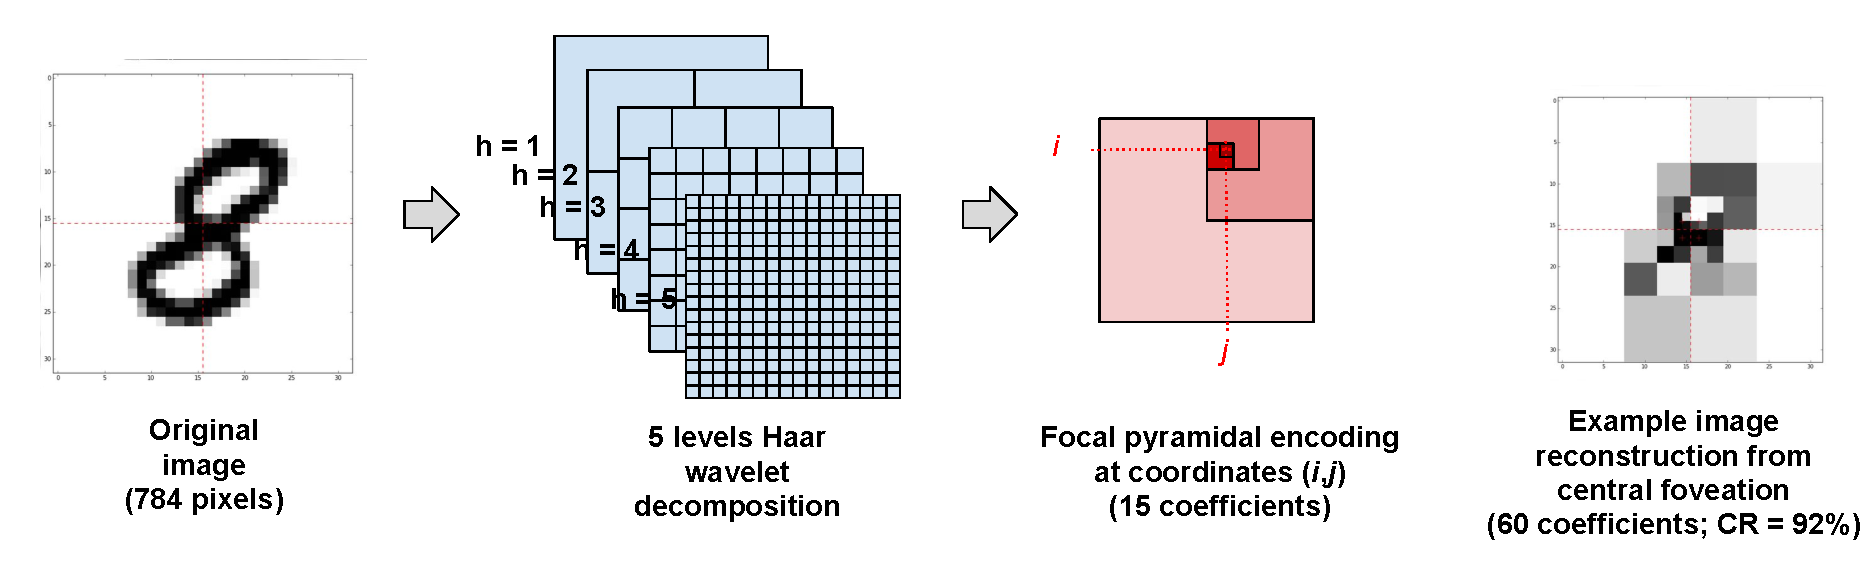
\includegraphics[width = \linewidth]{img/ICLR-foveated-model.pdf} 
	}
	
	\caption{\textbf{a}--\textbf{c}. Foveal ``pyramidal'' encoding from image. \textbf{a}. An original MNIST sample is recast on a $32\times32$ grid. \textbf{b}. It is then decomposed in a five levels Haar wavelets decomposition  issuing a total of 1024 wavelet coefficient. \textbf{c}. Then, for each gaze orientation $(i,j) \in \{0,...,15\}^2$, $3 \times 5$ wavelet coefficients are read out  at coordinates $(i,j)$, $(\lfloor\frac{i}{2}\rfloor,\lfloor\frac{j}{2}\rfloor)$,
	$(\lfloor\frac{i}{4}\rfloor,\lfloor\frac{j}{4}\rfloor)$,
	$(\lfloor\frac{i}{8}\rfloor,\lfloor\frac{j}{8}\rfloor)$	and
	$(\lfloor\frac{i}{16}\rfloor,\lfloor\frac{j}{16}\rfloor)$ in level descending order ).		
		\textbf{d}. Example image reconstruction from reading 60 central coefficients at coordinates (7,7), (7,8), (8,7) and (8,8), issuing a 92 \% compression rate.  
		}\label{fig:foveated}
\end{figure}

The baseline vision model we propose relies first on learning local foveated views on images.
Consistently with \citep{kortum1996implementation,wang2003foveation}, we restrain here the foveal transformation to its core algorithmic elements, i.e. the local compression of an image according to a particular focus. Our foveal image compression thus rests on a ``pyramid'' of 2D Haar wavelet coefficients placed at the center of sight. Taking the example of the MNIST database, we first transform the original images according to a 5-levels wavelet decomposition (see figure \ref{fig:foveated}b). We then define a viewpoint $\boldsymbol{u} = (i,j,h)$ as a set of 3 coordinates, with $i$ the row index, $j$ the column index and $h$ the spatial scale. Each $\boldsymbol{u}$ generates a visual field made of three wavelet coefficients $\boldsymbol{x}_{i,j,h} \triangleq\boldsymbol{x}|(i,j,h) \in \mathbb{R}^3$, obtained from an horizontal, a vertical and an oblique filter at location $(i,j)$ and scale $h$.  The multiscale visual information $\boldsymbol{x}_{i,j}\triangleq\boldsymbol{x}|(i,j) \in \mathbb{R}^{15}$ available at coordinates $(i,j)$ corresponds to a set of 5 coefficient triplets, namely $\boldsymbol{x}_{i,j}=\{\boldsymbol{x}_{i,j,5}, \boldsymbol{x}_{\lfloor i/2\rfloor,\lfloor j/2\rfloor,4}, \boldsymbol{x}_{\lfloor i/4\rfloor,\lfloor j/4\rfloor,3}, \boldsymbol{x}_{\lfloor i/8\rfloor,\lfloor j/8\rfloor, 2}, \boldsymbol{x}_{\lfloor i/16\rfloor,\lfloor j/16\rfloor, 1}\}$ (see figure \ref{fig:foveated}c), so that each multiscale visual field owns 15 coefficients (which is a radical compression when the 784 pixels of the original image are considered).
Fig. \ref{fig:foveated}d displays a reconstructed image from the 4 central viewpoints at coordinates (7, 7), (7, 8) (8, 7) and (8, 8).

\paragraph{Algorithms}

The generic sequential scene decoding setup is provided in algorithms \ref{algo:saccade-policy} and \ref{algo:saccade}. A significant algorithmic add-on when compared with formula
(\ref{eq:predictive-policy}) is the use of a \emph{dynamic actions set} : $\mathcal{U}$. At each turn, the new selected action $\tilde{u}$ is drawn off from $\mathcal{U}$, so that the next choice is made over fresh directions that have not yet been explored. This implements the inhibition of return principle stated in \citep{itti2001computational}. A second algorithmic add-on is the use of a threshold $H_\text{ref}$ to stop the evidence accumulation process when enough evidence has been gathered. This threshold is a free parameter of the algorithm that sets whether we privilege a conservative (tight) or optimistic (loose) threshold. The stopping criterion needs to be optimized to arbitrate between resource saving and decoding accuracy. 


\begin{algorithm}[t]
	\caption{Prediction-Based Policy}\label{algo:saccade-policy}
	\begin{algorithmic}
		\REQUIRE  $p$ ({\color{Purple}emission density}),  $\rho$ (prior), $A$ (objective function), $\mathcal{U}$ (actions set)
		%\STATE predict $z \sim \rho$
		\FOR{$\boldsymbol{z},\boldsymbol{u} \in \mathcal{Z,U}$}
		\STATE predict: $\tilde{\boldsymbol{x}}_{z,u} \sim p(X|\boldsymbol{z},\boldsymbol{u})$
		\STATE $r(\boldsymbol{z},\boldsymbol{u}) \leftarrow A(\boldsymbol{z},\boldsymbol{u},\tilde{\boldsymbol{x}}_{z,u},p,\rho)$ 
		\ENDFOR
		\RETURN $\tilde{\boldsymbol{u}} = \underset{\boldsymbol{u} \in \mathcal{U}}{\text{argmax }} \langle\rho, r(:,\boldsymbol{u})\rangle$
	\end{algorithmic}
\end{algorithm}

\begin{algorithm}[t]
	\caption{Scene Exploration}\label{algo:saccade}
	\begin{algorithmic}
		\REQUIRE  $p$ ({\color{Purple}emission density}), $\rho_0$ (initial prior), $A$ (objective), $\mathcal{U}$ (actions set)
		\STATE $\rho \leftarrow \rho_0$ 
		\WHILE {$H(\rho) > H_\text{ref}$}
		\STATE choose: $\tilde{\boldsymbol{u}} \leftarrow \text{Prediction-Based Policy}(p, \rho, A, \mathcal{U})$
		\STATE read: $\boldsymbol{x}_{\tilde{u}}$
		\STATE update: $\text{odd} \leftarrow \log p(\boldsymbol{x}_{\tilde{u}}|Z, \tilde{\boldsymbol{u}}) + \log \rho$ 
		\STATE $\rho \leftarrow \text{softmax} (\text{odd})$ \COMMENT{\emph{the posterior becomes the prior of the next turn}}
		\STATE $\mathcal{U} \leftarrow \mathcal{U} \setminus \{\tilde{u}\}$ 
		\ENDWHILE
		%		\RETURN $\rho$
	\end{algorithmic}
\end{algorithm}

The actual saccade exploration algorithm moreover adapts algorithm \ref{algo:saccade} the following way. The process starts from a loose assumption based on reading the root wavelet coefficient of the image, from which an initial guess $\rho_0$ is formed. Then, each follow-up saccade is {\color{Purple} defined as the gaze end-orientation} $(i,j) \in [0,..,15]^2$. {\color{Purple}In the pyramidal scene decoding case}, the posterior calculation rests on several coefficient triplets. After selecting gaze orientation $(i,j)$, all the corresponding coordinates $(i,j,h)$ are discarded from $\mathcal{U}$ and can not be reused for upcoming posterior estimation (for the final posterior estimate may be consistent with a uniform scan over the wavelet coefficients). 

\begin{figure}[t!]
	%\centerline{
	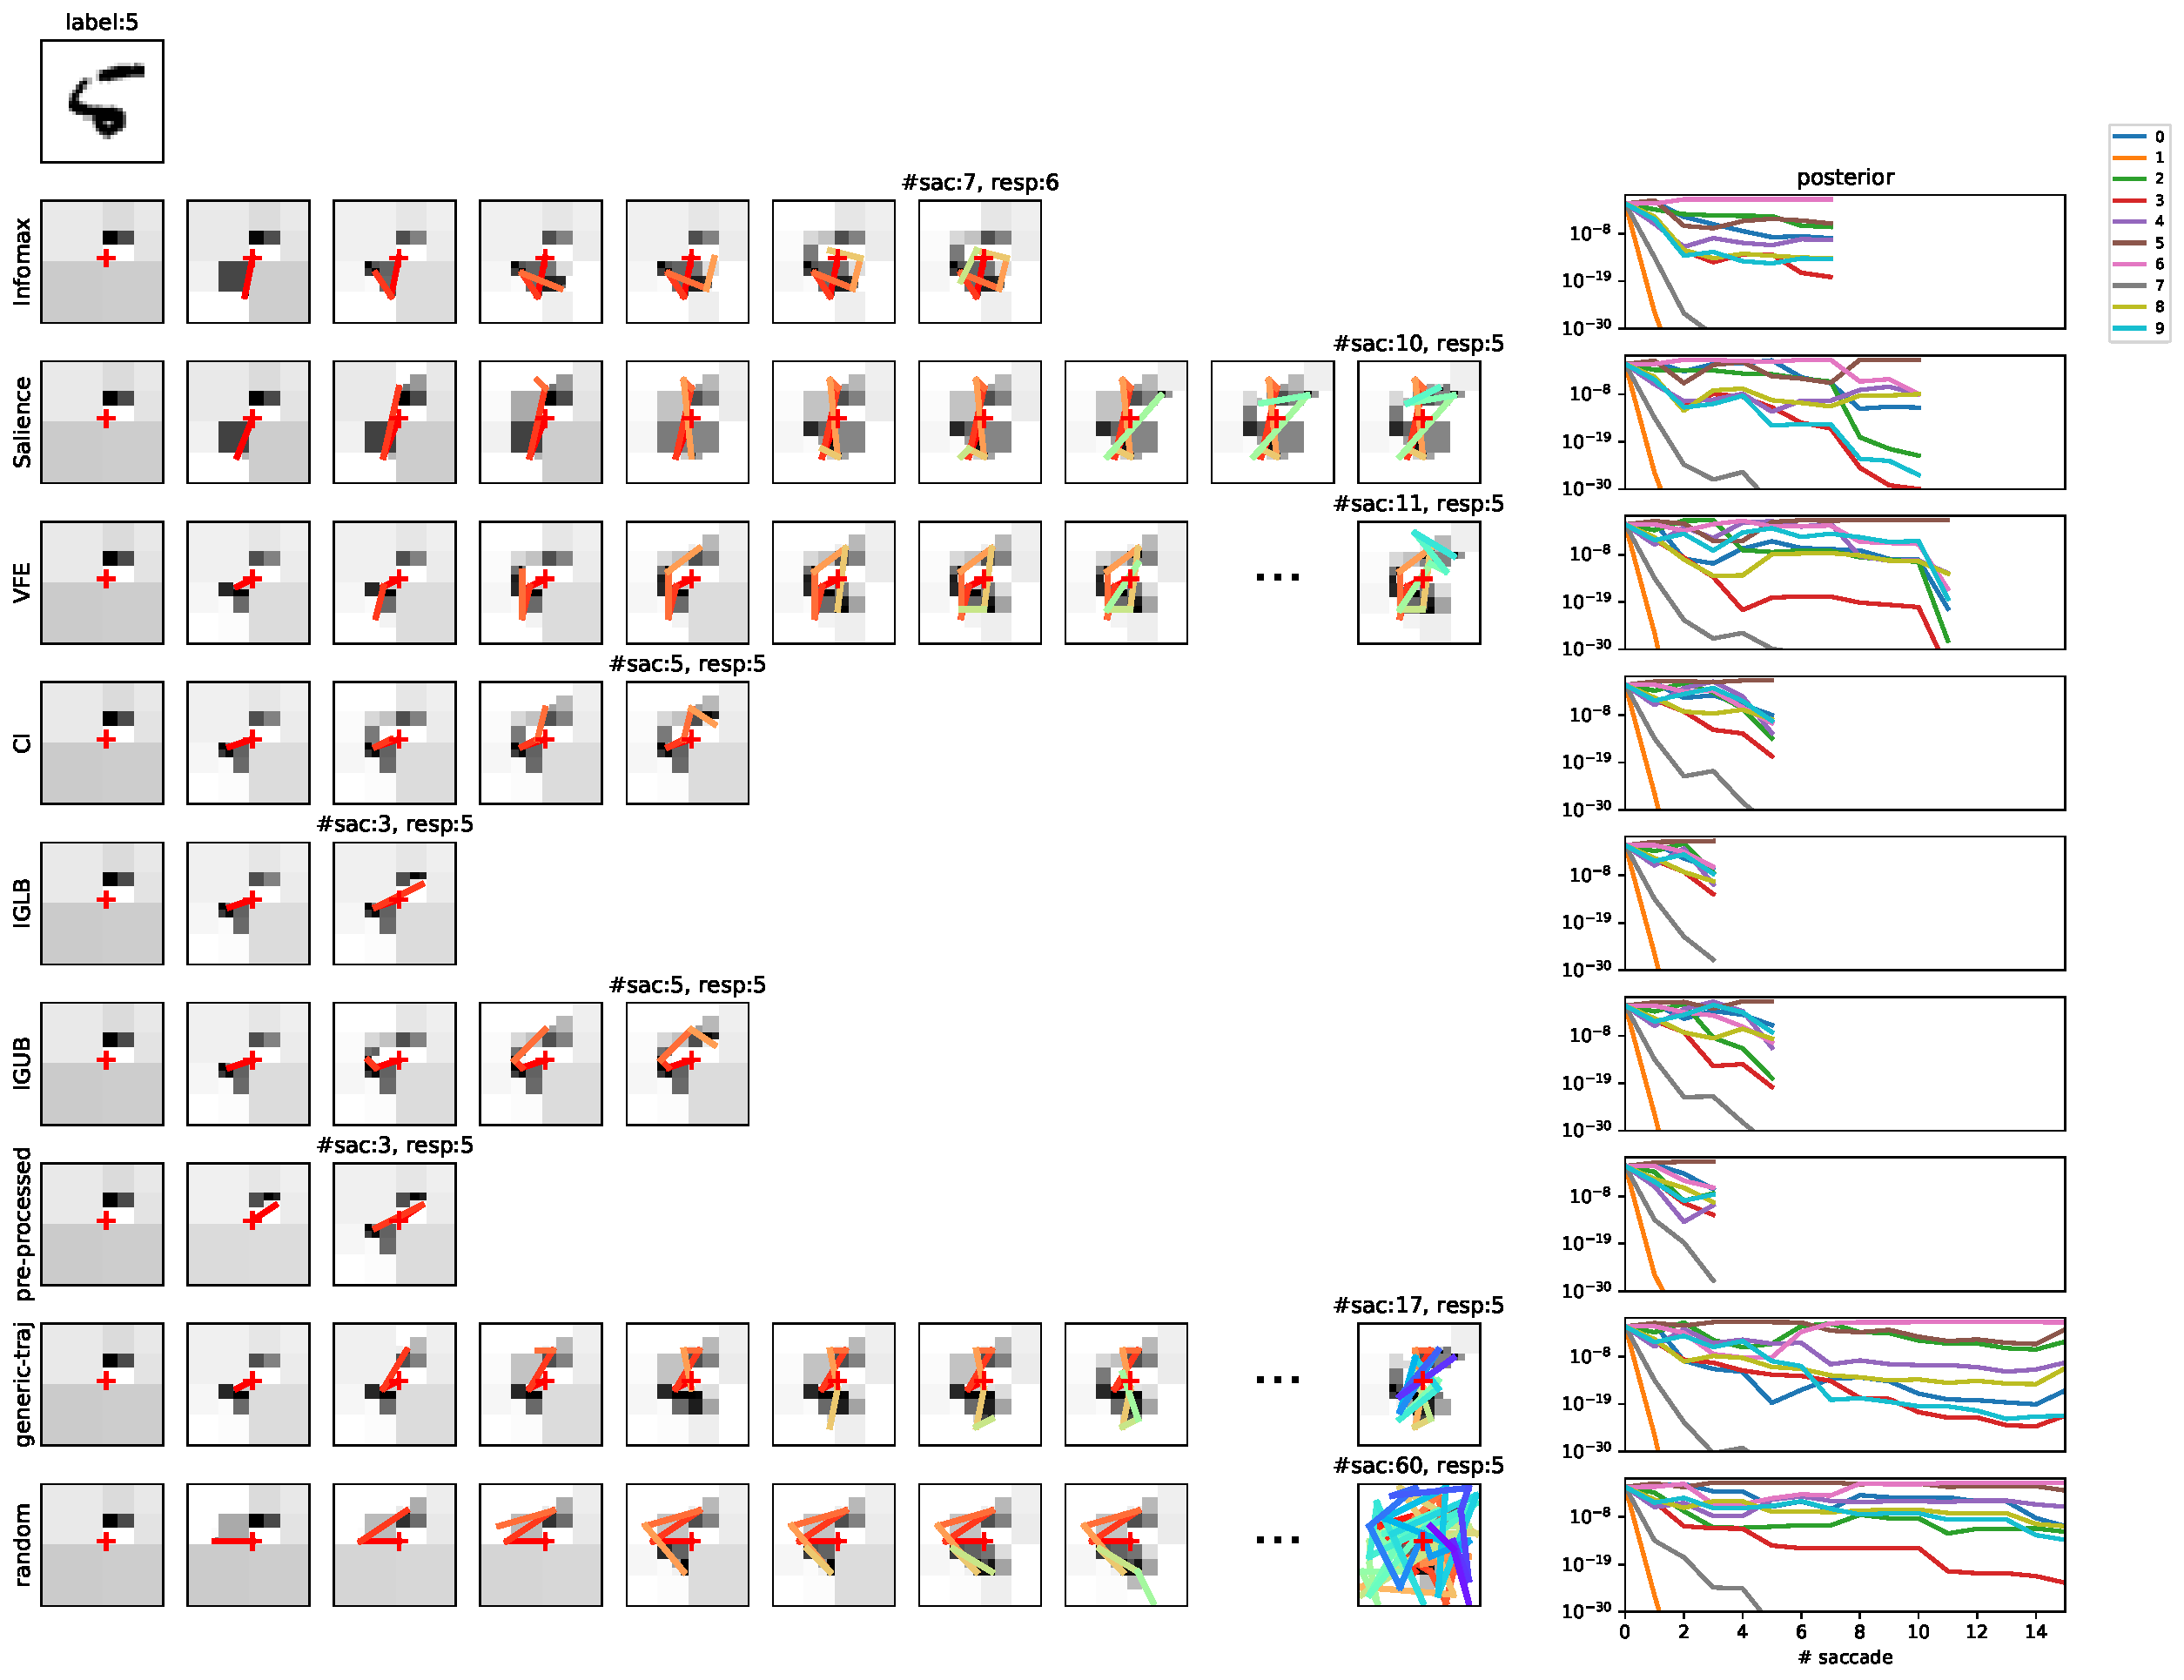
\includegraphics[width=\linewidth]{img/frontiers_trajectories_0.pdf}
	%}

	\caption{\textbf{Scene exploration through saccades in the foveated vision model}.\textbf{ Top left} : original MNIST sample to be decoded, with corresponding label. \textbf{Left panel} : Course of saccades for different action selection metrics. Leftmost is the policy name. For each row, the number of thumbnails reflects the number of saccades.  The scene decoding reads from left to right: more wavelet coefficients are grabbed at each step, visually reflected in an increased reconstruction neatness. On overlay is the corresponding sequence of visual fixations (with rainbow time color code). The number of saccades can vary for the different policies. Over the final thumbnail is the number of saccades and the final response. All decoding steps are shown except when $n>10$. \textbf{Right panel}: posterior update in function of the number of decoding steps, for $0 \leq n \leq 15$ (logarithmic y scale, one color per competing label). Baseline model (eq.~\ref{eq:bernouilli-gated}); $H_\text{ref} = 10^{-4}$. }\label{fig:foveated-saccades}
\end{figure}

\begin{figure}[t!]
	\centerline{
		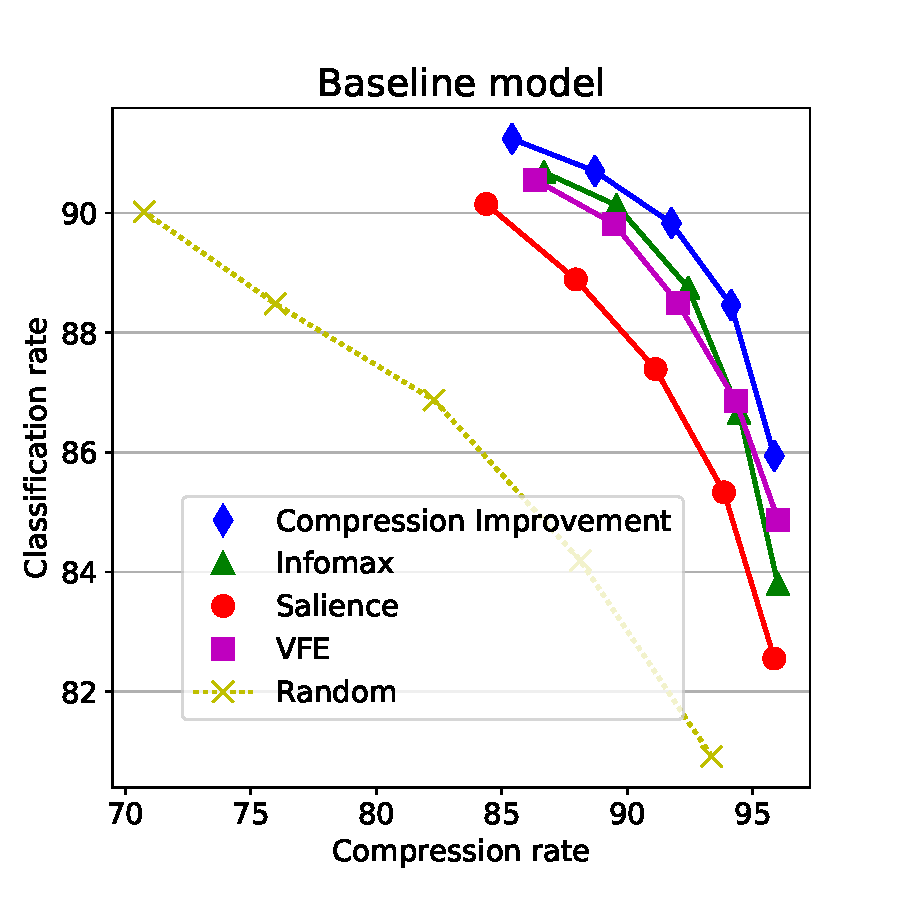
\includegraphics[width=.5\linewidth]{img/frontiers-classif-base.pdf}
		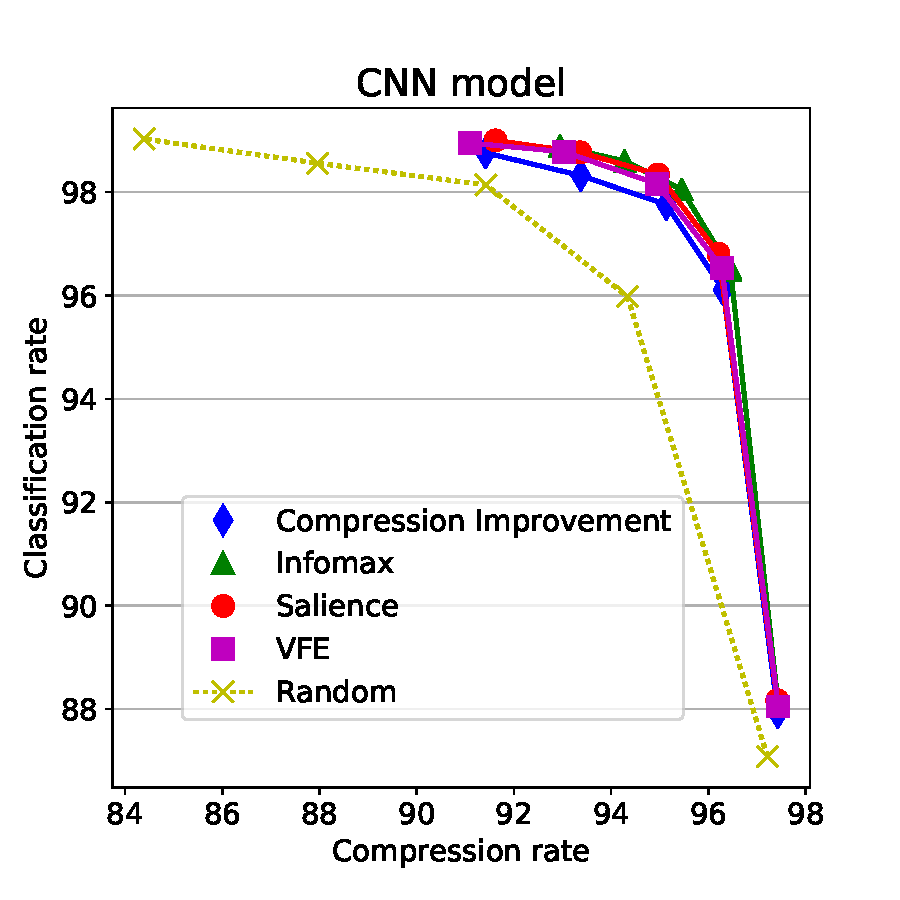
\includegraphics[width=.5\linewidth]{img/frontiers-classif-CNN.pdf}}
\caption{\textbf{Objective functions comparison.} The classification rates and average compression rates are processed after 10,000 sequential scene decoding sessions on the MNIST test set, with different objective (or loss) functions and different values of $H_\text{ref}$.  The classification rate is shown in function of the decoding compression rate. \textbf{Left:} Baseline model, with recognition threshold $H_\text{ref}$ varying from $10^{-5}$ up to  $H_\text{ref}=10^{-1}$ (from left to right). \textbf{Right:} CNN model, with recognition threshold varying from $H_\text{ref}=10^{-2}$ up to  $H_\text{ref}=1$ (from left to right).}
\label{fig:policy-comp-base}
\end{figure}

\paragraph{Baseline generative model and decoding compression}
A generative model is learned for each $\boldsymbol{u} = (i,j,h)$ (making a total of 266 data models) over the 55,000 examples of the MNIST training set. For each category $\boldsymbol{z}$ and each viewpoint $\boldsymbol{u}$, a generative {\color{Purple} emission} model is built over parameter set $\Theta_{\boldsymbol{z},\boldsymbol{u}} = (\rho_{\boldsymbol{z},\boldsymbol{u}}, \boldsymbol{\mu}_{\boldsymbol{z},\boldsymbol{u}}, \boldsymbol{\Sigma}_{\boldsymbol{z},\boldsymbol{u}})$, so that 
\begin{align}
\forall \boldsymbol{z},\boldsymbol{u}, \tilde{\boldsymbol{x}}_{\boldsymbol{z},\boldsymbol{u}} \sim
p(X|\boldsymbol{z},\boldsymbol{u}) =  \mathcal{B}(\rho_{\boldsymbol{z},\boldsymbol{u}}) \times \mathcal{N}(\boldsymbol{\mu}_{\boldsymbol{z},\boldsymbol{u}}, \boldsymbol{\Sigma}_{\boldsymbol{z},\boldsymbol{u}})\label{eq:bernouilli-gated}
\end{align} 
with $\mathcal{B}$ a Bernouilli distribution and $\mathcal{N}$ a multivariate Gaussian. The role of the Bernouilli is to ``gate'' the multivariate Gaussian model in the high frequencies, where digit deformations is reflected in an alternating presence or absence of pixels for high level coefficients and at the periphery, allowing to discard the ``white'' triplets from the Gaussian moments calculation. Each resulting emission density $p(X|Z,\boldsymbol{u})$ is a mixture of Bernouilli-gated Gaussians over the 10 MNIST labels. On the {\color{Purple}inference} side, the posterior is explicitly calculated using Bayes rule, i.e. $q(Z|\boldsymbol{x},\boldsymbol{u}) = \text{softmax} \log p(\boldsymbol{x}|Z,\boldsymbol{u})$, issuing about 92\% recognition rate on the MNIST test set when combining the 266 log likelihoods of each wavelet triplet of the full images with eq.~(\ref{eq:accum}), a typical recognition rate for shallow models.

\subsubsection{Metrics comparison in model-based scene decoding setups}

\paragraph{Baseline model}
Different examples of a sequential scene decoding are presented in figure \ref{fig:foveated-saccades} for one MNIST sample using algorithm \ref{algo:saccade} and different objective functions.
%The original image is presented in fig~\ref{fig:foveated-saccades}\textbf{a} with on overlay a four ``saccades'' trajectory over the image. The corresponding decoding process is illustrated in figs~\ref{fig:foveated-saccades}\textbf{b}--\textbf{e}, giving the reconstructed pixels from  coefficients read-out at successive steps of the decoding process.
Note that several coefficient triplets are read at each end-effector position ($i,j$) (see fig. \ref{fig:foveated}c). There is for instance a total of 5 triplets read out at the initial gaze orientation, and between 1 and 4 triplets read-out for each continuing saccade. 

Last, the \emph{decoding compression rate} is defined as the proportion of wavelet coefficients that are bypassed for reaching decision. In fig.~\ref{fig:foveated-saccades} first row for instance, a total of 25 coefficient triplets is  actually read-out, representing about 10\% of the total 256 coefficient triplets, issuing a 90\% decoding compression rate. 
The left-hand side of fig.~\ref{fig:policy-comp-base} shows how the classification rates vary in function of the decoding compression rate, for different objective functions and recognition threshold $H_\text{ref} \in \{10^{-1}, 10^{-2}, 10^{-3}, 10^{-4}, 10^{-5}\}$. The objectives are also compared with a random baseline policy. The classification rates monotonically increase with an \emph{decreasing} recognition threshold. Considering 92\% as the upper bound here, a near optimal recognition rate is obtained  at $H_\text{ref}=10^{-5}$ for the CI objective. Though all objectives functions show a consistent increase of the classification rate with decreasing $H_\text{ref}$, the CI{\color{Purple}-based policy} here overtakes the others {\color{Purple}policies}. The Infomax and the VFE{\color{Purple}-based policies} behave in a close-by fashion, and then the Salience{\color{Purple}-based policy} {\color{Purple} provides a less effective scene decoding}. 
{\color{Purple} All scene decoding policies provide elevated} compression rates, with a close to optimal classification obtained at around 85\% compression of the original data. It needs to be noticed that still a correct 90\% classification rate can be obtained with a random {\color{Purple} policy} at around 70\% compression rate, reflecting a strong redundancy in the original images.  

\begin{figure}
	\centerline{
		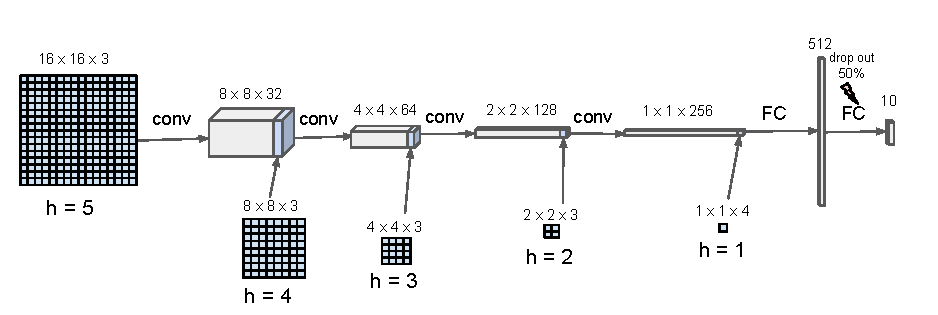
\includegraphics[width = \linewidth]{img/frontiers-convolutional.pdf} 
	}
	\vspace{-.2cm}
	\caption{\textbf{Hierarchical Convolutional Neural Network for Scene Decoding}. The CNN is composed of four convolutional layers and one fully connected layer. The input wavelet hierarchical organization is reflected in scale-dependent input inlay, consistently with stride-2 convolutional spatial integration.  }\label{fig:CNN}
\end{figure}

\paragraph{Convolutional Neural Network}
A convolutional neural network (CNN) was designed in order to provide a more effective {\color{Purple} inference} and facilitate comparison with state-of-the-art classifiers (see fig.~\ref{fig:CNN}). 
It is made of five convolution layers having each a distinct input corresponding to the five hierarchical levels of the wavelet decomposition. 
The CNN is biasless, uses a (2,2) stride for the convolutions \emph{without max-pooling}, promoting \emph{neighbour independence} in the convolutional computation track.
%The training data was compressed at random by discarding wavelet coefficient triplets, with a varying compression rate. 
Rectified Linear Units are used in all layers, except for the final layer owning linear units. 

The network was trained during about $10^6$ epochs with Tensorflow on a laptop.
{\color{Purple} Sparse foveal-consistent inputs are used for the training. For each training example, many gaze orientation $(i_1,j_1), ..., (i_n,j_n)$ are chosen at random, mimicking a $n$-views foveal visual scan, with $n$ randomly set from interval $\{1,..,256\}$. The multi-level input maps are then fed with the corresponding wavelet coefficients triplets, “pyramidally” distilled from $h = 5$ to $h = 0$.} {\color{Purple} The final network is expected to perform recognition on \emph{compressed} images, for which some wavelet coefficients are kept and some wavelet coefficients are discarded.} With standard parameter tuning { \color{Purple}(Adam optimizer \citep{kingma2014adam} with a learning rate equal to $10^{-4}$)}, the network attains a 99\% recognition rate on the test set with non-{\color{Purple}sparse} wavelet transformed inputs {\color{Purple}(full information case)}. 


The cross-entropy loss used in training {\color{Purple} allows to interpret} the network output as {\color{Purple} approaching} the data log-likelihood {\color{Purple}(up to a constant), i.e. $\text{CNN}(\boldsymbol{x}_{i,j}) \simeq \log p(\boldsymbol{x}_{i,j}|Z,(i,j)) + c$}. For decoding a scene, the input layers are initialized at zero  and progressively filled with new wavelet coefficients {\color{Purple} obtained during the scene exploration}.
The output is updated by adding supplementary data at the input only, complementing the data that was previously read, {\color{Purple} with $\exp \left[\text{CNN}(\boldsymbol{x}^{(1:n)}|\boldsymbol{u}^{(1:n)})\right] \propto p(\boldsymbol{x}^{(1:n)}|Z,\boldsymbol{u}^{(1:n)}) \propto p(Z|\boldsymbol{x}^{(1:n)},\boldsymbol{u}^{(1:n)}) = q^{(n)}$.} The posterior update is thus implemented \emph{from the data}. There is no recurrence, sequential accumulation or memory implemented in the network (like in eq.~\ref{eq:accum-post}). %{\color{magenta} like e.g. Bengio + nips review ref.}. 


Following algorithm \ref{algo:saccade} with the CNN as the {\color{Purple} approximate cumulated posterior estimator}, the decoding efficacy is shown for different objective functions on the right-hand side of  fig.~\ref{fig:policy-comp-base}. {\color{Purple} It is to be noted the CNN is only used for estimating the $q^{(n)}$'s posterior distributions, with the baseline Bernouilli-gated multivariate Gaussian model (eq.~\ref{eq:bernouilli-gated}) used on the predictive/generative side}. A clear decoding improvement is obtained {\color{Purple} when compared with the left-hand side of fig.~\ref{fig:policy-comp-base}}, with higher classification rates with less signal, attaining about 98,8\% correct classification with less than 8\% of the original image. Still, the general good performances of the decoder blurs the differences between the different policies. All objectives appear here equally good at effectively decoding the scene {\color{Purple} (except for the random action selection policy)}. 

\paragraph{Faulty model and failure robustness}
Predictive policies {\color{Purple}are known to heavily rest} on the generative models, that makes them sensible to model flaws. Resistance to model flaws is thus a property that should be prioritized when acting in unknown or coarsely modeled environments, or in the course of learning. In contrast with CNN-based optimal decoding, a failed probabilistic model was designed by simply setting $\rho_{u,z} = 1$ in eq.~(\ref{eq:bernouilli-gated}).  This tends to overestimate the signal strength at high frequencies, predicting a dense signal in effectively sparse regions. The classification accuracies are presented on fig.~\ref{fig:failed}\textbf{a} for the different objective functions considered here. In complement to the Compression Improvement (eq.~\ref{eq:CI}), the two variants referred as the IG Lower Bound (eq.~\ref{eq:PCI-n-1}) and the IG Upper Bound (eq.~\ref{eq:PC}) are also considered. 

The faulty model allows here to nicely separate the different objectives with regards to their optimistic vs. conservative flavor. While the CI is here barely  better than a random sampling, its conservative and optimistic variants respectively do clearly better and clearly worst than random exploration. The VFE loss and the Saliency objectives, as expected, amplify this effect with a strong robustness to model flaws for the VFE loss and, at reverse, a dramatic sensitivity  to model flaws for the Saliency objective. The Infomax also falls here in the optimistic category for its blindness to sequential consistency makes it update the posterior the wrong way.

\begin{figure}
	\centerline{{\bf a} \hspace{5.6cm} {\bf b}\hspace{5.6cm} {\bf c}}
	\centerline{
		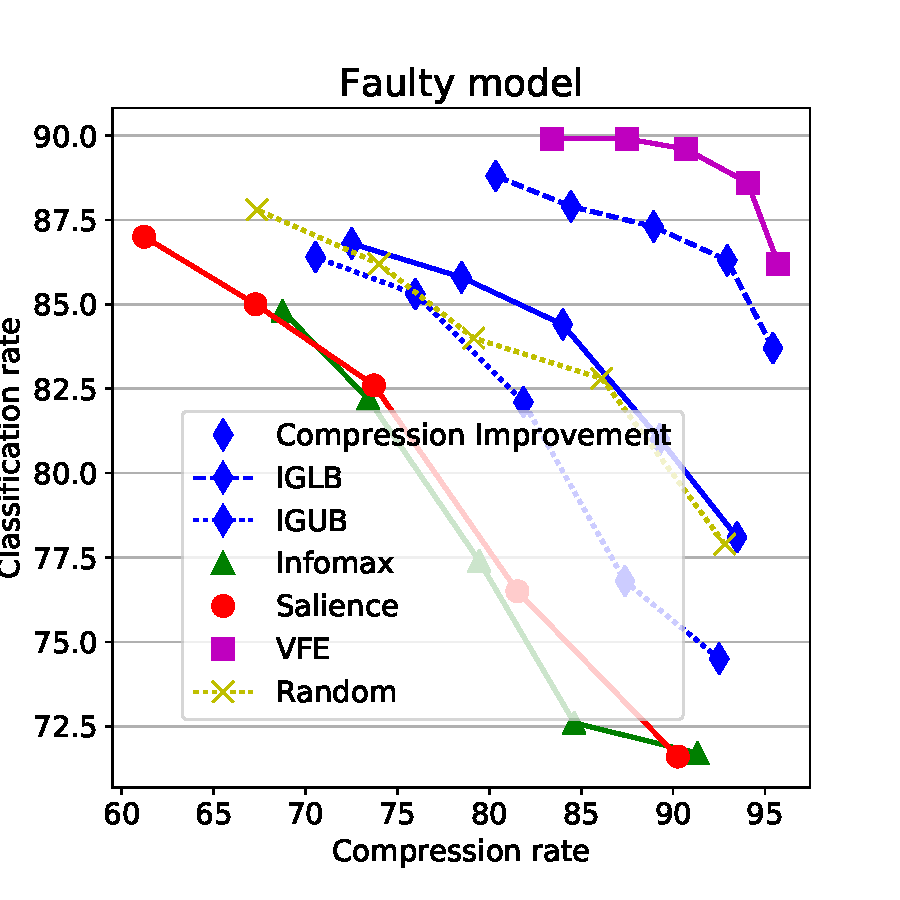
\includegraphics[width = .33\linewidth]{img/frontiers-classif-faulty.pdf} 
		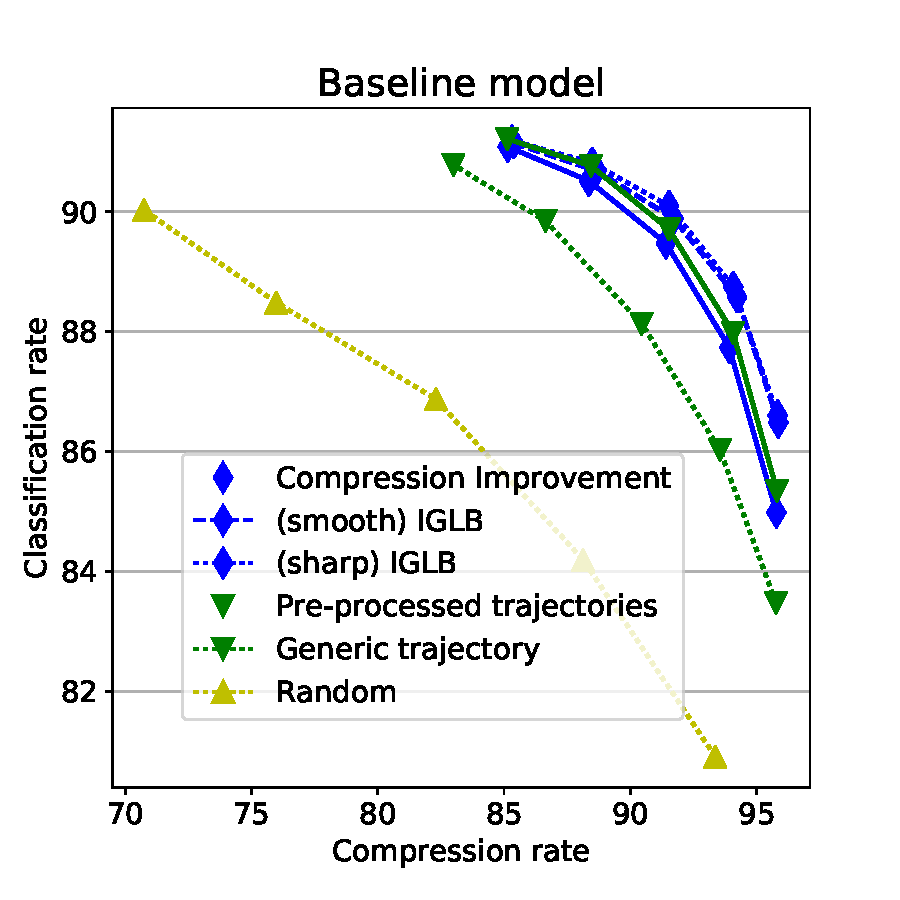
\includegraphics[width = .33\linewidth]{img/frontiers-classif-base-scaleup.pdf} 
		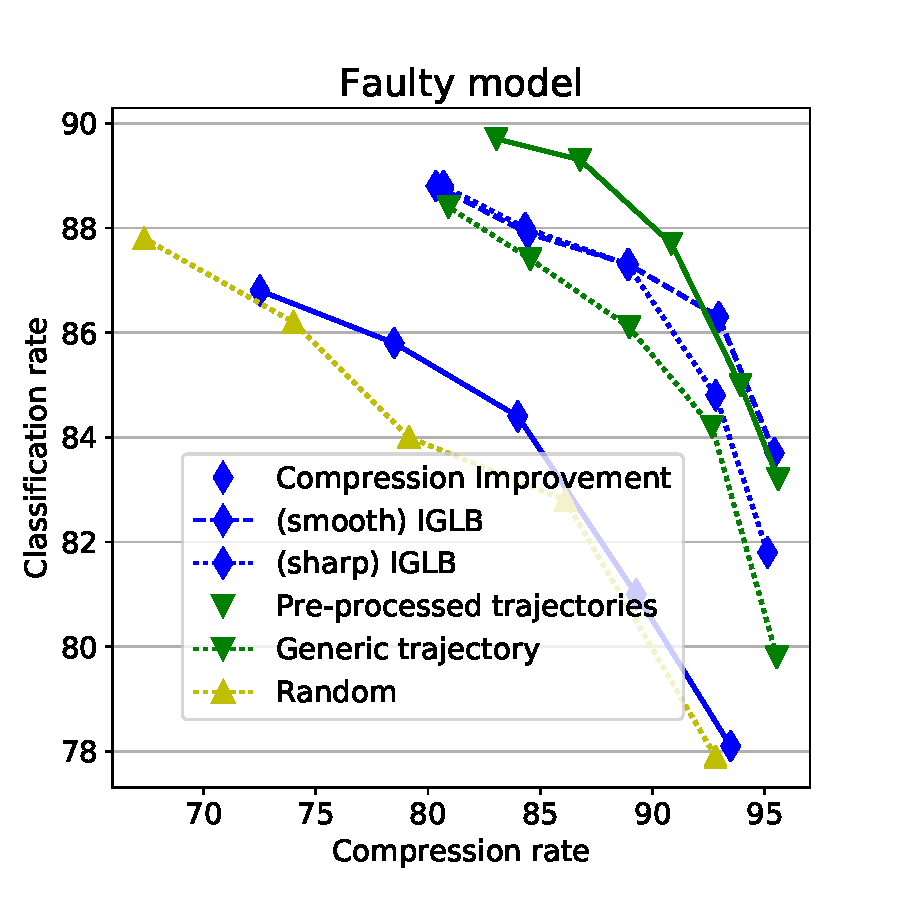
\includegraphics[width = .33\linewidth]{img/frontiers-classif-faulty-scaleup.pdf} 
			}
	\vspace{-.2cm}
	\caption{\textbf{Method comparisons}. \textbf{a}. Objective functions  comparison in a faulty model (see  fig.~\ref{fig:policy-comp-base}).  \textbf{b}. Information Gain-based computational schemes compared on the baseline model. \textbf{c}. Information Gain-based computational schemes compared on the faulty model. The recognition threshold varies from $H_\text{ref}=10^{-5}$ up to  $H_\text{ref}=10^{-1}$ (from left to right).}\label{fig:failed}
\end{figure}

\begin{figure}
	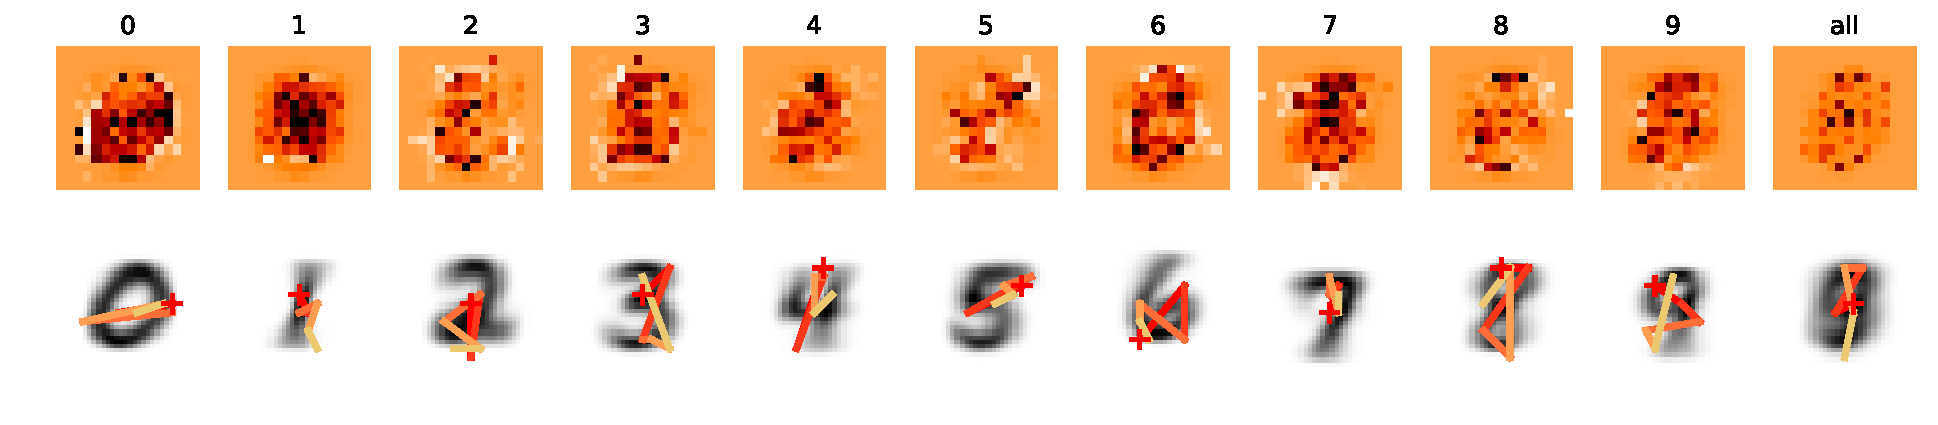
\includegraphics[width=\linewidth]{img/frontiers_sal_maps.pdf}
	\caption{\textbf{Pre-processed trajectories}. \textbf{Upper row (except rightmost map)}: color-coded pre-processed class-consistent log-posterior maps for $\boldsymbol{z} \in \{0,..,9\}$, for $\boldsymbol{u}$, on the baseline generative model, with low (whitish) to high (brownish) color-code. \textbf{Upper row, rightmost map:} Class-independent expected IGLB map.
	\textbf{Lower row:} Corresponding visual scan-path (the red ``+'' provides the initial gaze orientation). 5 first saccades shown, with average class prototype in the background. The rightmost background image is the average over all classes.}\label{fig:pre-processed}
\end{figure}

\subsubsection{Scaling up IG computation}
The scaling of the model needs to be addressed when large control spaces are considered. All predictive policies rely on a mixed encoding setup that implies to consider all $\boldsymbol{u}$'s and all $\boldsymbol{z}$'s in the prediction, which scales like $O(|\mathcal{U}|\times|\mathcal{Z}|^2)$ when the predicted posterior is needed in the objective/loss calculation, which is the case for the Infomax, the Saliency, the VFE the CI and the IGUB (algorithm \ref{algo:saccade-policy}), and $O(|\mathcal{U}|\times|\mathcal{Z}|)$ in the {\color{Purple}IGLB} case for it can bypass the posterior calculation. A quadratic cost may still be considered too heavy in real-case applications, implying to consider cheaper setups. 

\begin{itemize}
	\item A first simplification, referred as the ``sharp'' IGLB in  figs.~\ref{fig:failed}\textbf{b} and \ref{fig:failed}\textbf{c}, only samples a single $\boldsymbol{z}$ from $q^{(n-1)}$, i.e.: 
	$$ \hat{\boldsymbol{z}} = \underset{\boldsymbol{z}}{\text{argmax }} q^{(n-1)}(\boldsymbol{z})$$
	which makes the predictive policy scale like $O(|\mathcal{U}|)$. 
	\item An additional simplification can be obtained when considering the IGLB objective alone (eq.~\ref{eq:PCI-n-1}), for it is, on contrary to all other objectives, independent of the context $q^{(n-1)}$. For a given model $p$, and for all $\boldsymbol{z} \in \mathcal{Z}$, all the predictive log posteriors $\log p(\boldsymbol{z}|\hat{\boldsymbol{x}}_{z,u}, \boldsymbol{u})$ can be pre-processed using the \emph{mode} of the predicted visual field $\hat{\boldsymbol{x}}_{z,u} = \underset{\boldsymbol{x}}{\text{ argmax }} p(\boldsymbol{x}|\boldsymbol{z}, \boldsymbol{u})$ as a sample. {\color{Purple} This results in a set of class-consistent log posterior maps providing, for each $\boldsymbol{u} \in \mathcal{U}$, the expected log posterior value $\log p(\hat{\boldsymbol{z}}|\hat{\boldsymbol{x}}_{\hat{z},u}, \boldsymbol{u})$, given prior assumption $\hat{\boldsymbol{z}} = \underset{\boldsymbol{\boldsymbol{z}}}{\text{ argmax }} q^{(n-1)}(\boldsymbol{z})$ (fig.~\ref{fig:pre-processed}, first row)}. Then, for each assumption $\boldsymbol{z}$,  a class-specific visual exploration strategy can be \emph{pre-processed}. Given an assumption $\boldsymbol{z}$, a pre-processed trajectory can be defined, following a log-posterior descending order over the $\boldsymbol{u}'s$, {\color{Purple} from higher IGLB values of toward lower IGLB values (brownish toward whitish in fig.~\ref{fig:pre-processed})}.  $|\mathcal{Z}|$ saccade trajectories of size $|\mathcal{U}|$ are then stored  in a set of $\boldsymbol{z}$-indexed ordered lists, with a $O(|\mathcal{U}|\times|\mathcal{Z}|)$ memory load but only $\simeq O(1)$ readout computational cost. 
	In practice, the viewpoint selected at step $n$ depends on the current guess $\hat{\boldsymbol{z}}$, with on-the-fly pre-processed trajectory switch if the guess is revised across the course of saccades. This strategy is referred a the \emph{pre-processed trajectories} in figs~\ref{fig:foveated-saccades}, \ref{fig:failed}\textbf{b} and \ref{fig:failed}\textbf{c}. 
	\item For comparison, a \emph{generic} trajectory was also computed using \begin{align}
	\overline{\text{IGLB}}(\boldsymbol{u})
	= \mathbb{E}_{\boldsymbol{z} \sim p(Z)}\left[ \log p(\boldsymbol{z}|\hat{\boldsymbol{x}}_{z,u}, \boldsymbol{u})\right]
	\end{align} with a uniform prior over the $\boldsymbol{z}'s$, i.e. $p(\boldsymbol{z}) = \frac{1}{|\mathcal{Z}|}$.
	It is referred a the \emph{generic trajectory} in figs~\ref{fig:foveated-saccades}, \ref{fig:failed}\textbf{b} and \ref{fig:failed}\textbf{c}.
\end{itemize}

{\color{Purple} The log-posterior maps allow to analyze in detail the class-consistent orientations (that appear brownish) as opposed to the class-inconsistent orientations (pale orange to white). First to be noticed is the relative scarceness of the class-consistent orientations. 
	%Those "evidence providing" locations appear, as expected, mutually exclusive from class to class. 
A small set of saccades is expected to provide most of the classification information while the rest of the image is putatively uninformative (or even counter informative if whitish). A second aspect is that the class-relevant locations are all located in the central part of the images, so there is very few chance for the saccades to explore the periphery of the image where little information is expected to be found. This indicates that the model has captured the essential concentration of class-relevant information in the central part of the images for that particular training set.}

The different simplification strategies are compared in figs~\ref{fig:failed}\textbf{b} and \ref{fig:failed}\textbf{c} over the baseline and the faulty models. Both the sharp IGLB and the pre-processed trajectories are shown consistent with the CI objective on fig.~\ref{fig:failed}\textbf{b}, despite their considerably lower computational cost, while the generic trajectory strategy appears less effective. Interestingly, those computational simplifications also remain valid when robustness to model flaws is considered (fig.~\ref{fig:failed}\textbf{c}). 
Both the sharp IGLB and the pre-processed trajectories allow to reach both robustness and effective classification rates at considerably lower cost than the ``smooth'' IGLB.


\section{Conclusion}
A generic fovea-based scene decoding setup was presented which, accordingly with \citep{najemnik2005optimal}, rests on a predictive decoding accuracy to choose action. A variational approach to scene encoding is adopted, which, accordingly with \citep{friston2012perceptions}, optimizes the data reconstruction cost by picking new sensory samples through action. In our case, the visual field is interpreted under a \emph{mixed encoding} setup for the visual data is both generated by the viewpoint and the scene constituents. 
This allows to unify the many objective functions proposed in the literature under a single master objective referred as the Compression Improvement in \citep{schmidhuber2007simple}, that is shown to provide a consistent interpretation for most of the objective functions used in perception-driven control. Two variants of the CI objective are proposed, using either the pre-sample or the post-sample posterior in the approximation. In the pre-sample case, it is shown to be an Information Gain Lower Bound objective that always underestimate the actual Information Gain. Following the IGLB objective is thus expected to lower the risk of failed interpretation in the case of failed predictions. Using the Variational Free Energy \citep{friston2015active} as a loss (instead of the IGLB) is moreover expected to \emph{bias} the action selection in an even more conservative way. 
Conversely, the Information Gain Upper Bound objective (IGUB) is shown to always \emph{overestimate} the actual Information Gain. Following the IGUB objective is thus expected to increase the risk of failed interpretation in the case of failed predictions. 
Using the Saliency objective \citep{itti2005bayesian} instead of the IGUB is moreover expected to \emph{bias} the action selection in an even more optimistic way, subsequently increasing the failed scene interpretation risk.

The presented numerical experiments thus highlight different aspects of the setup. 
A first and principal result is that state-of-the-art recognition rates can be obtained with sequential fovea-based computation using less than 10\% of the original signal. This strong input compression is made possible for the visual data owns lot of redundancies that are not used at their best in computer vision, doing useless computations over large parts of the visual scene. The general good results obtained in that case reflect the advantage of mixing a predictive controller with accurate state-of-the-art predictors, here a deep neural network. 

A second result is the sub-optimality of many classical objective function widely used in literature, like the ``Infomax'' \citep{butko2010infomax} and the ``Salience'' objectives \citep{itti2005bayesian}, when the scene decoding setup is considered. Their sub-optimality is not manifest with finely-tuned generative models, but becomes patent when a coarse of faulty model is used.
This may appear counter-intuitive at first sight for the Infomax objective is vastly dominant in predictive control \citep{najemnik2009simple}, while the Salience objective provides among the best predictions for human fixation zones \citep{itti2005bayesian}. The mixed performances of the Salience objective in predictive control may however be attenuated when learning is considered. Heading toward inconsistently modeled places is indeed a sensible behaviour when the model is to be updated. This entails maximizing predictions errors, which is a relevant principle long considered in sparse reinforcement learning \citep{schmidhuber1991curious,oudeyer2008can,pathak2017curiosity}. The main difference lies in considering model-based predictive rewards, as we do here, versus model-free post-hoc rewards. In the second case, an \emph{observed} inconsistency reflects a model flaw that needs to be adressed, while in the first case, it only reflects a predictive inconsistency, that is part of the model, favoring oblivious rather than memory-consistent scene interpretation. This trade-off between predictive versus post-hoc reward reflects more generally a profound contradiction between exploiting at best the current knowledge and past observations versus challenging the current interpretation to leverage conflicting facts, a variant of the exploration/exploitation trade-off. 

Last, a notorious defect of the predictive setup is its computational cost scaling with the size of the actions sets, that may grow combinatorially fast with increasing degrees of freedom. Real-world predictive control is thus in need for computationally-effective predictive models, here attainable with the Information Gain Lower Bound (IGLB) objective, that, though maximizing the Information Gain in approximation, is independent from the current state of interpretation. In discrete interpretation spaces, it is thus possible to pre-process prototypic trajectories following a guess-confirmation sequence of actions, that can be read-out from memory without computationally-demanding predictions. This dramatically simplified setup is shown efficient in our case, showing both competitive decoding compression rates and good robustness to model flaws. 
%and ways toward cheap and scalable predictive policies.  

\subsection*{Acknowledgements}
{\color{magenta}\bf Thanks to Laurent Perrinet XXXXXXXXXXXXXXXXXXXXXXXXXXXXXXXXX...}

\appendix

\section{View-dependent variational encoding setup}\label{app:VFE}
{\color{Purple} 
	%In a model-based approach, the latent variable $\boldsymbol{z}$ is expected to specify the state of the physical environment. In the model-free case, only weak assumptions need to be made about the latent space.  The latent space $\mathcal{Z}$ just needs to be expressive enough to capture and restore all necessary information about the environment.  
	The \emph{variational encoding} perspective \citep{hinton1994autoencoders} was originally developed 
	to train unsupervised autoencoder neural networks. 
	%The general idea is that an efficient code is a code that is both compact and accurate at restoring the data. 
	If $\boldsymbol{x}$ is the original data, the corresponding code $\boldsymbol{z}$ is generated by a distribution $q$, i.e. $\boldsymbol{z} \sim q(Z)$. This distribution is called the \emph{encoder}. Then, the reconstruction is made possible with a second conditional probability over the codes, i.e. $p(X|\boldsymbol{z})$, that is called the \emph{decoder}. If $\boldsymbol{z}$ is the current code, the reconstructed data is $\tilde{\boldsymbol{x}} \sim p(X|\boldsymbol{z})$. 
	
	In short, the efficacy of a code is estimated by an information-theoretic quantity, the ``reconstruction cost'' that is defined for every $\boldsymbol{x}$ knowing $p$ and $q$:
	\begin{align}
	F(\boldsymbol{x}) %&= - \sum_{\boldsymbol{z} \in \mathcal{Z}} q(\boldsymbol{z}) \log (p(\boldsymbol{x}|\boldsymbol{z})p(\boldsymbol{z})) - H(q)\nonumber\\
	%&= \mathbb{E}_{z\sim q} \left[-\log (p(\boldsymbol{x}|\boldsymbol{z})p(\boldsymbol{z}))\right] - H(q)
	%\label{eq:FEP-energy}\\
	&= \mathbb{E}_{z\sim q} \left[-\log (p(\boldsymbol{x}|\boldsymbol{z}))\right] +\text{KL}(q(Z)||p(Z))
	\label{eq:FEP-prior}\\
	&= - \log p(\boldsymbol{x}) + \text{KL}(q(Z)||p(Z|\boldsymbol{x}))
	\label{eq:FEP}
	\end{align}
	%with $\mathcal{Z}$ an arbitrary encoding space, $q$ an arbitrary distribution over the codes, $H(q) = -\sum_z q(\boldsymbol{z}) \log q(\boldsymbol{z})$ the entropy of $q$, $p(X|Z)$ the decoder and $p(Z)$ a prior distribution over the codes.
	%The densities $p$ and $q$ are called ``variational'' for they can be optimized according to the data \citep{hinton2006fast,kingma2013auto}.  
	with $p(Z)$ the prior over the latent state.
	$F$ is also said the Variational Free Energy (VFE), for it shares shares a mathematic analogy with the Helmhotz Free Energy \citep{friston2010free}.
	%It can then be shown, with some reordering, that:
	%
	%so that an optimal encoder $q(Z)\simeq p(Z|\boldsymbol{x})$ can be approached through a stochastic gradient descent over $p$ and $q$ according to $-\nabla_{p,q} F(\boldsymbol{x}) $	 --~see \citep{kingma2013auto}~-- so that the reconstruction cost should meet the ``description length'' of the data, i.e. its estimated (natural) Shannon Information under the model $p$:
	%\begin{align*}
	%h(\boldsymbol{x}) \simeq -\log p(\boldsymbol{x}) \simeq  F(\boldsymbol{x})
	%\end{align*}
	%that is a quantity representing how unlikely $\boldsymbol{x}$ is regarding the data model $p$. 
	Minimizing the cost $F$ according to $p$ and $q$ thus means minimizing the ``surprise'' caused by observing the data $\boldsymbol{x}$ \citep{friston2010free}.
	
	\paragraph{View-dependent VFE}
	If we now turn back to the viewpoint selection setup, an additional factor $\boldsymbol{u}$ (the viewpoint) comes into the play. The data $\boldsymbol{x}$ that is actually read is now conditioned on  $\boldsymbol{u}$, so that:
	\begin{align}
	F(\boldsymbol{x}|\boldsymbol{u}) 
	%&= \mathbb{E}_{z\sim q} \left[-\log (p(\boldsymbol{x}|\boldsymbol{z},\boldsymbol{u})p(\boldsymbol{z}))\right] - H(q)\\
	&= \mathbb{E}_{z\sim q} \left[-\log (p(\boldsymbol{x}|\boldsymbol{z},\boldsymbol{u}))\right] +\text{KL}(q(Z)||p(Z))
	\label{eq:FEP-prior-u-app}\\
	&= - \log p(\boldsymbol{x}|\boldsymbol{u}) + \text{KL}(q(Z)||p(Z|\boldsymbol{x}, \boldsymbol{u}))
	\label{eq:FEP-posterior-u-app}\end{align}
}

When only the variations of $p$ and $q$ are considered in the optimization, each viewpoint $\boldsymbol{u}$ provides a distinct optimization problem that is resolved by finding $q(Z)\simeq p(Z|\boldsymbol{x}, \boldsymbol{u})$. Each $\boldsymbol{u}$ may thus drive a different posterior and thus a different reconstruction cost. It is thus feasible to change (and optimize) the reconstruction cost through changing $\boldsymbol{u}$.

\paragraph{Sequential VFE}
{\color{Purple} 
	When generalized to many observations: $(\boldsymbol{x},\boldsymbol{u}), (\boldsymbol{x}',\boldsymbol{u}')$, ..., $(\boldsymbol{x}^{(n)},\boldsymbol{u}^{(n)})$, the $n^\text{th}$ reconstruction cost $F^{(n)}(\boldsymbol{x}^{(n)}|\boldsymbol{u}^{(n)}, ..., \boldsymbol{x}, \boldsymbol{u})$ also obeys to the chain rule (see eq.~\ref{eq:accum-post}), i.e. is estimated from $q^{(n-1)}$, $\boldsymbol{u}^{(n)}$ and $\boldsymbol{x}^{(n)}$ only:
	\begin{align}
	F(\boldsymbol{x}^{(n)}|\boldsymbol{u}^{(n)}; q^{(n-1)}) 
	&= \mathbb{E}_{\boldsymbol{z} \sim q} \left[-\log p(\boldsymbol{x}^{(n)}| \boldsymbol{z}, \boldsymbol{u}^{(n)} )\right] + \text{KL}(q(Z)||q^{(n-1)}(Z))
	\label{eq:FEP-prior-uxun-app}\\
	&= -\log p(\boldsymbol{x}^{(n)}|\boldsymbol{u}^{(n)}) + \text{KL}(q(Z)||p(Z|\boldsymbol{x}^{(n)},\boldsymbol{u}^{(n)};q^{(n-1)}))
	\label{eq:FEP-posterior-uxun-app}
	\end{align}
	with %$q^{(n)}$ the shared (or cumulative) encoding according to the past and current observations, and 
	$q^{(n-1)}$ having the role of the prior, providing a \emph{forward} variational encoding scheme (see also \citep{chung2015recurrent,fraccaro2016sequential}.  
	
\bibliographystyle{apalike}
\bibliography{biblio}



\end{document}